% ─────────────────────────────────────────────────────────────────────────────
\chapter{Results and Operational Robustness Analysis}
\label{chap:results}
% ─────────────────────────────────────────────────────────────────────────────

This chapter presents the experimental results of the \gls{fairlab} evaluation
pipeline, with particular attention to the operational robustness of
\gls{ai}-based systems for image classification and triage in forensic
contexts. The analysis does not aim to construct an absolute ranking based
solely on accuracy, but rather to evaluate how proxy models and selected
black-box software systems react to clean inputs, \gls{ood} samples,
anti-forensic transformations, and adversarial perturbations. The interpretation
of the results therefore maintains an explicitly forensic focus, considering
false negatives on the \texttt{weapon} class, the tendency to force \gls{ood}
inputs into known operational classes, the traceability of the bundle, the
normalization of black-box outputs, and the continued need for human
review~\cite{costantini2019digital,sanna2024preliminary,sanna2025pixelperfect}.


% ─────────────────────────────────────────────────────────────────────────────
\section{Experimental Evaluation Scope and Dataset Overview}
\label{sec:results-scope}
% ─────────────────────────────────────────────────────────────────────────────

This chapter reports the results obtained by applying the \gls{fairlab}
protocol described in Chapter~\ref{chap:methodology}. The evaluation is
organized into two complementary levels. The first level concerns the proxy
models, for which architectures, checkpoints, predictions, confidence scores,
confusion matrices, and aggregate metrics are available. The second level
concerns the selected black-box software systems, for which the evaluation is
based exclusively on observable outputs, normalized exports, and matching
against the experimental ground truth.

The objective of this chapter is not to construct an absolute ranking among
proxy models and selected software systems, nor to transform the thesis into an
\gls{advml} benchmark. Rather, the focus is to evaluate the operational
robustness of \gls{ai}-based systems with respect to conditions that are
relevant to \gls{df} workflows: clean inputs, \gls{ood} samples,
anti-forensic transformations, adversarial perturbations, and processing
through selected software systems. From this perspective, particular importance
is assigned to false negatives on the \texttt{weapon} class, false positives on
\texttt{non\_weapon} content, behavior on out-of-distribution samples, and the
ability to trace each result back to the corresponding experimental artifact.

Table~\ref{tab:results-evaluation-scope} summarizes the final status of the
experimental components considered in this chapter.

\begin{table}[H]
\centering
\scriptsize
\renewcommand{\arraystretch}{1.15}
\setlength{\tabcolsep}{4pt}
\caption{Final scope of the experimental evaluation.}
\label{tab:results-evaluation-scope}
\begin{tabularx}{\textwidth}{@{}p{0.27\textwidth} p{0.22\textwidth} X@{}}
\toprule
\textbf{Component} & \textbf{Status} & \textbf{Role in Chapter~\ref{chap:results}} \\
\midrule

Final dataset &
\textbf{Frozen} &
1500 balanced images: 500 \texttt{weapon}, 500 \texttt{non\_weapon}, and
500 \texttt{ood}. \\

Binary subset &
\textbf{Frozen} &
1000 images: 500 \texttt{weapon} and 500 \texttt{non\_weapon}; used for the
clean baseline, adversarial perturbations, and anti-forensic transformations. \\

Clean splits &
\textbf{Completed} &
Five deterministic folds of 200 images each, with 100 \texttt{weapon} samples
and 100 \texttt{non\_weapon} samples per fold. \\

\gls{ood} set &
\textbf{Separated} &
500 images evaluated as an autonomous operational risk, not as a third
supervised class of the binary task. \\

Proxy models &
\textbf{Evaluated} &
EfficientNet-B0, ResNet18, and \gls{clip}; used for the controlled and
reproducible analysis of clean, \gls{ood}, adversarial, and anti-forensic
performance. \\

Adversarial attacks &
\textbf{Generated and evaluated} &
\gls{fgsm}, \gls{superdeepfool}, \gls{sigmazero}, \gls{onepixel}, and
\gls{colorshift}. \\

Anti-forensic transformations &
\textbf{Generated and evaluated} &
\gls{jpegrecompression}, \gls{resampleresize}, \gls{gaussianblur},
\gls{histogrammodification}, and \gls{contraststretching}. \\

Forensic evaluation bundle &
\textbf{Consolidated} &
11\,500 files prepared for the evaluation of the proxy models and selected
black-box software systems. \\

\gls{magnetaxiomtool} / \gls{magnetai} &
\textbf{Consolidated} &
Evaluated as a commercial forensic platform with \gls{ai}-based
categorization; the \texttt{Possible weapons} tag is recoded as a positive
\texttt{weapon} prediction. \\

\gls{excirefoto2025} &
\textbf{Consolidated} &
Evaluated as a standalone general-purpose semantic retrieval software
application with \gls{ai}-based functionality, under the operational
configurations \texttt{D20}, \texttt{D50}, and \texttt{D80}. \\

\gls{cellebriteinseyets} &
\textbf{Consolidated} &
Evaluated as a commercial black-box software platform for media analysis,
through observable outputs exported and normalized from the
\texttt{Cellebrite Physical Analyzer 10.9.0.3029} environment. \\

\gls{griffeye} / \gls{t3kcore} &
\textbf{Consolidated} &
Evaluated as a commercial black-box media triage platform, through automatic
semantic bookmarks generated by \gls{t3kcore}; the
\texttt{CORE/Violence/Firearm} bookmark is recoded as a positive
\texttt{weapon} prediction. \\

\gls{xai} &
\textbf{Integrated} &
Qualitative and diagnostic analysis through \gls{ig} on representative cases;
not used as a primary metric. \\

\bottomrule
\end{tabularx}
\end{table}

Table~\ref{tab:results-corpus-composition} reports the consolidated composition
of the experimental corpus used for the quantitative analyses. Clean,
adversarial, and anti-forensic samples are derived from the binary
\texttt{weapon}/\texttt{non\_weapon} subset. \gls{ood} samples, by contrast,
are kept separate: they are not used to compute supervised accuracy, but to
measure the tendency of systems to map out-of-distribution content to one of
the two operational classes.

\begin{table}[H]
\centering
\caption{Composition of the experimental corpus and forensic evaluation bundle.}
\label{tab:results-corpus-composition}
\begin{tabularx}{0.90\textwidth}{@{}l r X@{}}
\toprule
\textbf{Condition} & \textbf{Files} & \textbf{Role in the evaluation} \\
\midrule

Clean
&
1000
&
Nominal baseline on the binary \texttt{weapon}/\texttt{non\_weapon} subset. \\

\gls{ood}
&
500
&
Evaluation of out-of-distribution behavior; not treated as a third supervised
class. \\

Adversarial
&
5000
&
Five adversarial perturbations applied to the binary subset of 1000 images,
with 1000 files for each perturbation. \\

Anti-forensic
&
5000
&
Five model-agnostic transformations applied to the binary subset of 1000
images, with 1000 files for each transformation. \\

\midrule
\textbf{Total}
&
\textbf{11\,500}
&
Complete forensic evaluation bundle, used for the controlled evaluation of
proxy models and for the black-box evaluation of selected software systems. \\

\bottomrule
\end{tabularx}
\end{table}

The metrics reported in the following sections are derived from the files
produced by the experimental pipeline. For the proxy models, clean and
perturbed performance is derived from
\codepath{results/metrics/final_core_metrics.csv}, the confusion matrices from
\codepath{results/metrics/final_confusion_matrices.csv}, \gls{ood} behavior
from \codepath{results/metrics/final_ood_metrics.csv}, and robustness metrics,
including accuracy drop, induced errors, and confidence shift, from
\codepath{results/metrics/final_robustness_metrics.csv}. For the selected
software systems, the aggregate metrics are derived from
\codepath{results/metrics/forensic_tools_metrics.csv}, whereas normalized
predictions and audit checks are obtained from the corresponding normalized
exports in \codepath{evaluation/forensic_tools/}. The outputs of the black-box
software systems are therefore analyzed through a common representation that is
independent of the native export format.

An additional caution concerns the interpretation of confidence. The confidence
values reported for the proxy models are used as intra-model indicators and not
as calibrated probabilities directly comparable across different architectures.
This caution is even more relevant in the comparison with selected black-box
software systems, which do not necessarily expose numerical scores, decision
thresholds, or homogeneous uncertainty measures. For this reason, confidence is
used in this chapter as an auxiliary diagnostic element, not as a stand-alone
evidentiary measure.

In the remainder of the chapter, a single convention is adopted for computing
performance drop:
\[
\text{accuracy}_{\mathrm{drop}} =
\text{accuracy}_{\mathrm{clean}} - \text{accuracy}_{\mathrm{perturbed}}.
\]

Positive values therefore indicate performance degradation with respect to the
clean baseline; values equal to zero indicate stability; negative values
indicate a slight increase in accuracy under the perturbed condition. Such
increases, when present, are not interpreted as evidence of general robustness,
but as oscillations dependent on the sample distribution and on the specific
transformation applied.

The forensic evaluation bundle constitutes the operational connection between
the controlled experimental level and the selected black-box software level.
The blind view of the bundle allows the software systems to process the files
without direct exposure to labels, attack names, fold information, or
experimental metadata, whereas the manifests and \gls{sha256}/\gls{md5} hashes
make it possible to map each normalized output back to the corresponding
artifact. This approach makes it possible to distinguish among classification
errors, missed detections, uncategorized outputs, non-interpretable mappings,
and limitations specific to the export formats of individual software systems.


% ─────────────────────────────────────────────────────────────────────────────
\section{Clean Baseline Performance}
\label{sec:results-clean-baseline}
% ─────────────────────────────────────────────────────────────────────────────

Evaluation on clean inputs constitutes the experimental baseline against which
the behavior of the models under subsequent conditions must be interpreted,
namely \gls{ood} samples, anti-forensic transformations, and adversarial
perturbations. In this phase, the proxy models are evaluated on the official
binary subset composed of 1000 images, balanced between 500 \texttt{weapon}
samples and 500 \texttt{non\_weapon} samples. The positive class is defined as
\texttt{weapon}, whereas the negative class is defined as
\texttt{non\_weapon}; consequently, false negatives indicate
\texttt{weapon} samples classified as \texttt{non\_weapon}, while false
positives indicate \texttt{non\_weapon} samples classified as \texttt{weapon}.

Table~\ref{tab:results-clean-baseline-metrics} reports the main performance
metrics of the three proxy models on the clean binary subset. In addition to
accuracy, balanced accuracy, and macro-averaged metrics, the table also reports
the mean confidence associated with the predictions, which is useful for
distinguishing nominal performance from the level of confidence expressed by
the model.

\begin{table}[H]
\centering
\scriptsize
\setlength{\tabcolsep}{2.3pt}
\renewcommand{\arraystretch}{1.15}
\caption{Clean performance of the proxy models on the binary subset.}
\label{tab:results-clean-baseline-metrics}
\begin{tabularx}{\textwidth}{@{}l *{11}{>{\centering\arraybackslash}X}@{}}
\toprule
\textbf{Model} &
\textbf{Acc.} &
\textbf{Bal.} &
\textbf{M-P} &
\textbf{M-R} &
\textbf{M-F1} &
\textbf{P\textsubscript{w}} &
\textbf{R\textsubscript{w}} &
\textbf{F1\textsubscript{w}} &
\textbf{Conf.} &
\textbf{\acrshort{fpr}} &
\textbf{\acrshort{fnr}} \\
\midrule
EfficientNet-B0 & 0.978 & 0.978 & 0.978 & 0.978 & 0.978 & 0.972 & 0.984 & 0.978 & 0.979 & 0.028 & 0.016 \\
ResNet18 & 0.964 & 0.964 & 0.964 & 0.964 & 0.964 & 0.958 & 0.970 & 0.964 & 0.974 & 0.042 & 0.030 \\
\acrshort{clip} & 0.927 & 0.927 & 0.933 & 0.927 & 0.927 & 0.881 & 0.988 & 0.931 & 0.559 & 0.134 & 0.012 \\
\bottomrule
\end{tabularx}

\vspace{0.4em}
\footnotesize
\textit{Note.} \textit{Bal.} indicates balanced accuracy; \textit{M-P},
\textit{M-R}, and \textit{M-F1} indicate macro-precision, macro-recall, and
macro-F1, respectively; \(P_w\), \(R_w\), and \(F1_w\) indicate precision,
recall, and F1-score for the \texttt{weapon} class; \textit{Conf.} indicates
the mean confidence of the predictions.
\end{table}

EfficientNet-B0 achieves the highest nominal performance, with an accuracy of
0.978, a macro-F1 of 0.978, and a mean confidence of 0.979. ResNet18 shows
slightly lower but still high performance, with an accuracy of 0.964, a
macro-F1 of 0.964, and a mean confidence of 0.974. \gls{clip} achieves an
accuracy of 0.927 and a macro-F1 of 0.927, but exhibits a different
operational profile from the two supervised models: recall on the
\texttt{weapon} class is very high, at 0.988, whereas the \gls{fpr} is
substantially higher, at 0.134. Moreover, the mean confidence of \gls{clip} is
0.559, much lower than that observed for EfficientNet-B0 and ResNet18.

This behavior should not be interpreted as the effect of zero-shot
classification. In the adopted experimental protocol, \gls{clip} is used as a
pre-trained and frozen visual encoder, adapted to the
\texttt{weapon}/\texttt{non\_weapon} task through a supervised binary head. The
observed tendency to produce high recall on the \texttt{weapon} class, at the
cost of a higher \gls{fpr}, is therefore more appropriately interpreted as an
effect of the pre-trained visual representation and of the calibration of the
binary head with respect to the specific task, rather than as the result of a
zero-shot mechanism. The lower mean confidence also suggests that the greater
tendency to flag images as \texttt{weapon} does not necessarily correspond to
high-confidence predictions.

Table~\ref{tab:results-clean-confusion-matrices} reports the aggregate
confusion matrices for each model, using the layout
\(\left[\left[\gls{tn}, \gls{fp}\right], \left[\gls{fn}, \gls{tp}\right]\right]\).

\begin{table}[H]
\centering
\caption{Clean confusion matrices of the proxy models.}
\label{tab:results-clean-confusion-matrices}
\begin{tabular}{@{}l r r r r@{}}
\toprule
\textbf{Model} & \textbf{\gls{tn}} & \textbf{\gls{fp}} & \textbf{\gls{fn}} & \textbf{\gls{tp}} \\
\midrule
EfficientNet-B0 & 486 & 14 & 8 & 492 \\
ResNet18 & 479 & 21 & 15 & 485 \\
\gls{clip} & 433 & 67 & 6 & 494 \\
\bottomrule
\end{tabular}
\end{table}

The same error distribution is visualized in
Figure~\ref{fig:results-clean-confusion-matrices}, which highlights the
different operational profiles of the three models: EfficientNet-B0 minimizes
the total number of errors, ResNet18 maintains an intermediate behavior,
whereas \gls{clip} reduces false negatives on the \texttt{weapon} class at the
cost of a higher number of false positives.

\begin{figure}[htbp]
\centering

\begin{minipage}{0.48\textwidth}
\centering
\small EfficientNet-B0

\vspace{0.2em}
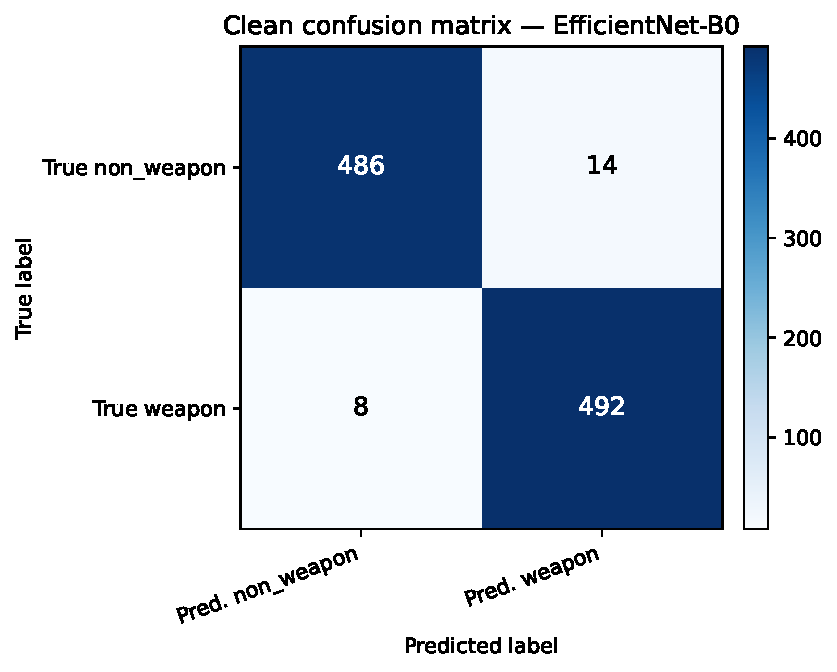
\includegraphics[width=\linewidth]{images/fig_clean_confusion_matrix_efficientnet_b0.pdf}
\end{minipage}
\hfill
\begin{minipage}{0.48\textwidth}
\centering
\small ResNet18

\vspace{0.2em}
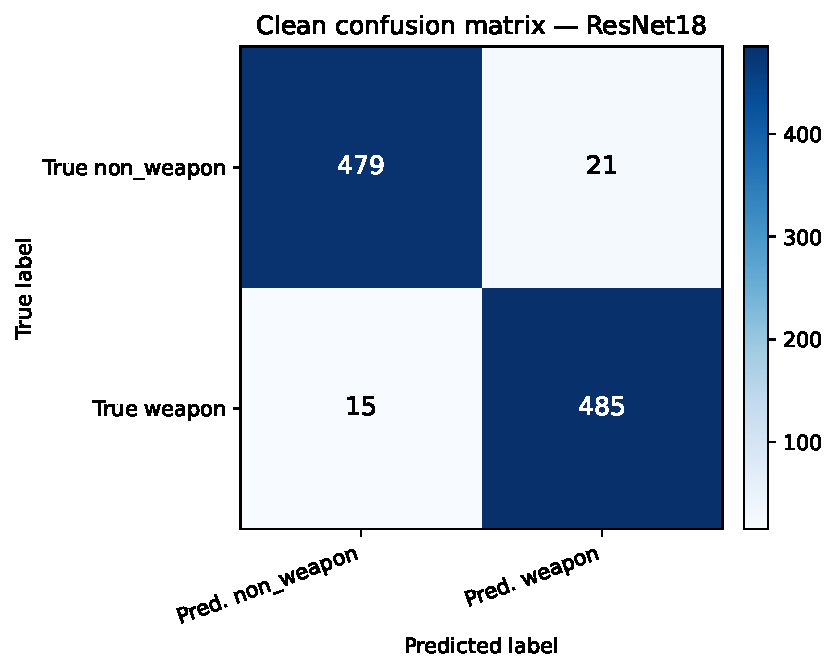
\includegraphics[width=\linewidth]{images/fig_clean_confusion_matrix_resnet18.pdf}
\end{minipage}

\vspace{0.8em}

\begin{minipage}{0.48\textwidth}
\centering
\small \acrshort{clip}

\vspace{0.2em}
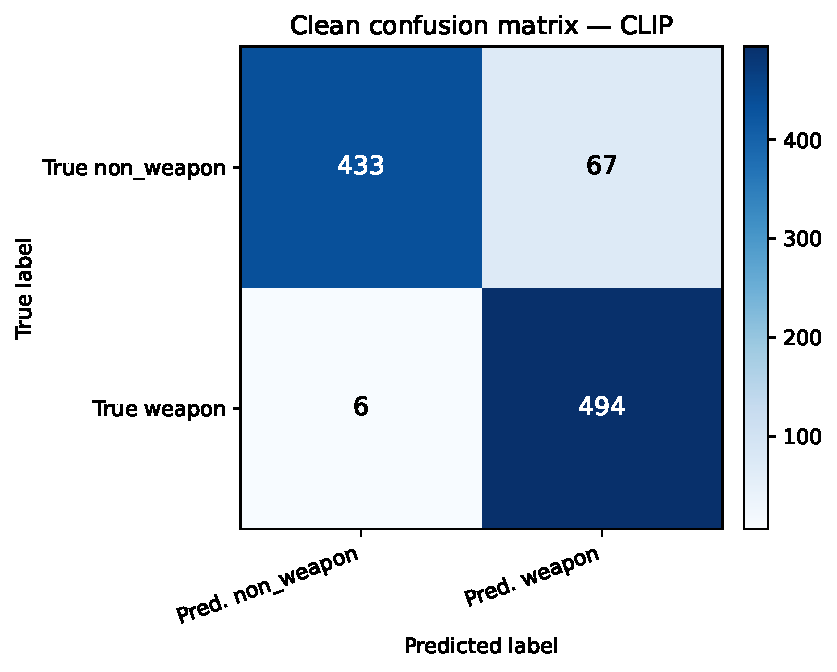
\includegraphics[width=\linewidth]{images/fig_clean_confusion_matrix_clip.pdf}
\end{minipage}

\caption{Clean confusion matrices of the three proxy models on the binary subset. Rows represent the true label, whereas columns represent the predicted label.}
\label{fig:results-clean-confusion-matrices}
\end{figure}

From a forensic perspective, the most critical figure is the number of false
negatives on the \texttt{weapon} class. EfficientNet-B0 produces 8 false
negatives, ResNet18 produces 15, whereas \gls{clip} produces 6. However,
\gls{clip} also produces 67 false positives, a substantially higher value than
the 14 produced by EfficientNet-B0 and the 21 produced by ResNet18.
Consequently, the clean comparison cannot be interpreted only in terms of
overall accuracy, but must also consider the different balance among
sensitivity to the investigatively relevant class, risk of improper flags, and
level of confidence associated with the predictions.

Overall, the clean baseline shows that the proxy models achieve high
performance under nominal conditions. However, the differences among accuracy,
\gls{fpr}, \gls{fnr}, and mean confidence already highlight, even in the
absence of perturbations, an aspect that is relevant for forensic triage:
models with similar accuracy may produce different operational risk profiles,
especially when the error concerns the failure to flag \texttt{weapon} content,
the improper classification of \texttt{non\_weapon} content as potentially
relevant, or the production of highly confident predictions on cases that still
require human verification.

% ─────────────────────────────────────────────────────────────────────────────
\section{Out-of-Distribution Behavior and False Positive Risk}
\label{sec:results-ood}
% ─────────────────────────────────────────────────────────────────────────────

The \gls{ood} evaluation analyzes the behavior of the proxy models on images
that do not belong to the nominal binary
\texttt{weapon}/\texttt{non\_weapon} task. These samples include borderline or
out-of-distribution content, such as knives, swords, replicas, airsoft items,
synthetic renderings, video game images, war scenes, military vehicles,
explosions, and degraded or anomalous images. Unlike adversarial perturbations
and anti-forensic transformations, the \gls{ood} condition does not represent an
attack, but a realistic operational risk: in an investigative workflow,
ambiguous images or images that do not fully adhere to the operational classes
of the model may still be submitted to automated analysis
\cite{hendrycks2017baseline,liang2018odin,fort2021exploring}.

The metrics are aggregated over 2\,500 predictions, obtained by evaluating the
500 \gls{ood} images through the five fold-aware checkpoints of each model.
This choice preserves consistency with the evaluation strategy adopted for the
binary subset, while maintaining the conceptual separation between \gls{ood}
samples and the \texttt{weapon}/\texttt{non\_weapon} task. The
\emph{weapon rate} indicates the proportion of \gls{ood} samples classified as
\texttt{weapon}; the \emph{high-confidence rate} indicates the proportion of
predictions with confidence of at least 0.9. In this section, these values must
not be interpreted as accuracy or supervised error on a third class, but as
indicators of the risk that out-of-distribution samples are operationally
absorbed into one of the two classes of the binary task.

\begin{table}[H]
\centering
\scriptsize
\setlength{\tabcolsep}{3.5pt}
\renewcommand{\arraystretch}{1.15}
\caption{Behavior of the proxy models on \gls{ood} samples.}
\label{tab:results-ood-behavior}
\begin{tabular}{@{}l r r r r r r r@{}}
\toprule
\textbf{Model} &
\textbf{Tot.} &
\textbf{Pred. w} &
\textbf{Pred. nw} &
\textbf{W-rate} &
\textbf{Conf.} &
\textbf{HC-count} &
\textbf{HC-rate} \\
\midrule
EfficientNet-B0 & 2\,500 & 924 & 1\,576 & 0.3696 & 0.8505 & 1\,252 & 0.5008 \\
ResNet18 & 2\,500 & 1\,094 & 1\,406 & 0.4376 & 0.8896 & 1\,617 & 0.6468 \\
\acrshort{clip} & 2\,500 & 2\,089 & 411 & 0.8356 & 0.5358 & 0 & 0.0000 \\
\bottomrule
\end{tabular}

\vspace{0.4em}
\footnotesize
\textit{Note.} \textit{Pred. w} indicates \texttt{weapon} predictions;
\textit{Pred. nw} indicates \texttt{non\_weapon} predictions;
\textit{W-rate} indicates the proportion of \gls{ood} samples classified as
\texttt{weapon}; \textit{Conf.} indicates mean confidence; \textit{HC-count}
indicates the number of predictions with confidence of at least 0.9;
\textit{HC-rate} indicates the corresponding proportion over the total
\gls{ood} predictions. The total of 2\,500 predictions per model is obtained by
evaluating the 500 \gls{ood} images through each of the five fold-aware
checkpoints.
\end{table}

The null \textit{HC-rate} value for \gls{clip} does not indicate the absence of
\texttt{weapon} classifications on \gls{ood} samples, but the absence of
predictions with confidence greater than or equal to the high-confidence
threshold fixed at 0.9. Indeed, \gls{clip} maps 83.56\% of the \gls{ood}
predictions to the \texttt{weapon} class, but with a mean confidence of 0.5358.
This behavior highlights a semantic tendency toward the \texttt{weapon} class
that is not accompanied by high-confidence predictions.

Figure~\ref{fig:results-ood-weapon-rate-confidence} visualizes the comparison
among weapon rate, mean confidence, and high-confidence rate, whereas
Figure~\ref{fig:results-ood-confidence-distribution} shows the distribution of
predictive confidence on \gls{ood} samples.

\begin{figure}[H]
\centering
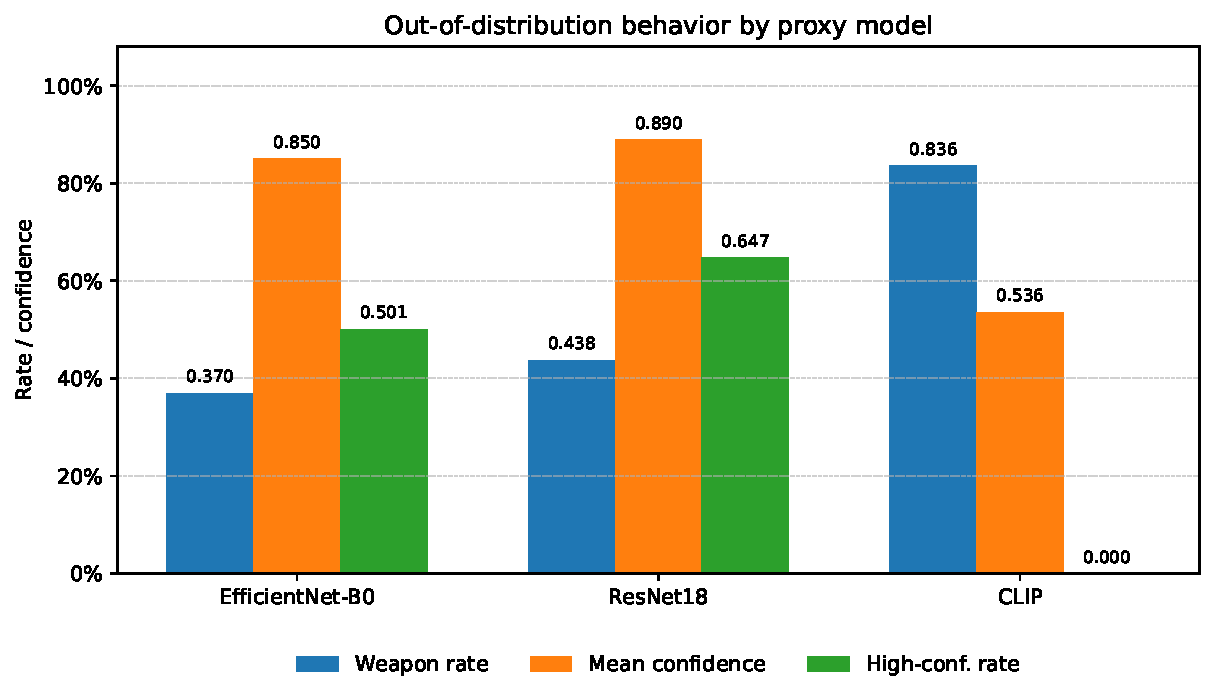
\includegraphics[width=0.88\textwidth]{images/fig_ood_weapon_rate_and_confidence.pdf}
\caption{Behavior of the proxy models on \gls{ood} samples: proportion of \texttt{weapon} predictions, mean confidence, and proportion of high-confidence predictions.}
\label{fig:results-ood-weapon-rate-confidence}
\end{figure}

The results show three distinct operational profiles. \gls{clip} classifies a
very high proportion of \gls{ood} samples as \texttt{weapon}, at 0.8356, but
does so with moderate mean confidence, at 0.5358, and with no predictions above
the high-confidence threshold. EfficientNet-B0 and ResNet18 classify lower
proportions of \gls{ood} samples as \texttt{weapon}, at 0.3696 and 0.4376,
respectively, but with much higher mean confidence values. In particular,
ResNet18 reaches the highest high-confidence rate, at 0.6468, whereas
EfficientNet-B0 reaches 0.5008.

\begin{figure}[H]
\centering
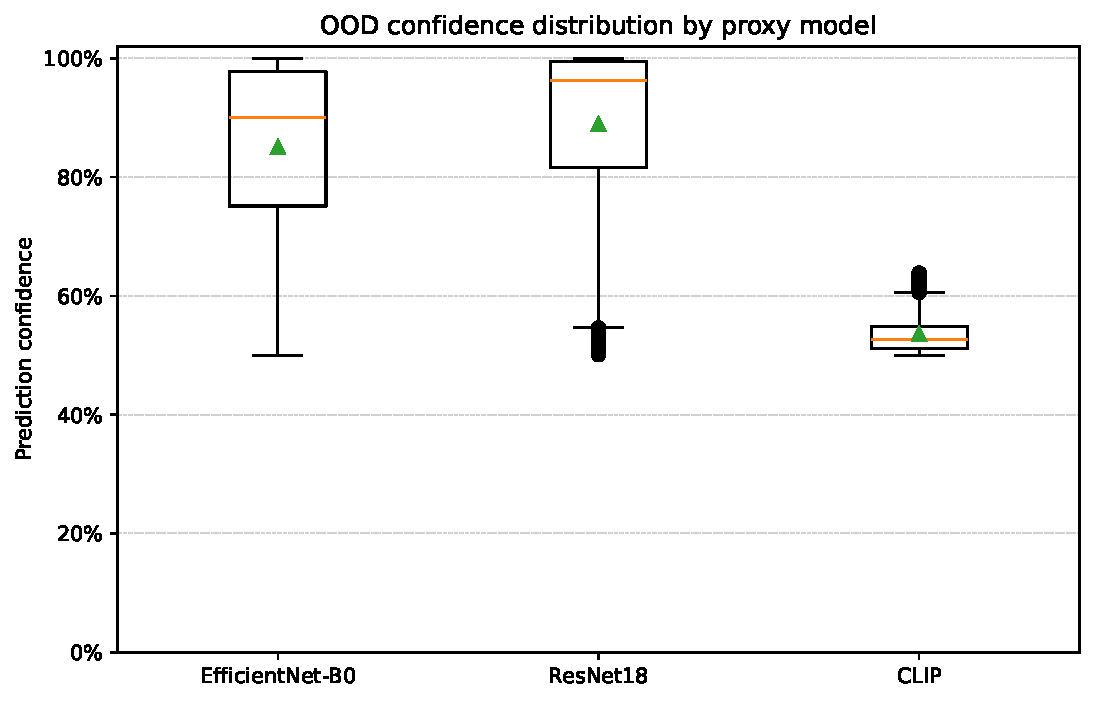
\includegraphics[width=0.82\textwidth]{images/fig_ood_confidence_distribution.pdf}
\caption{Distribution of predictive confidence on \gls{ood} samples for each proxy model. The plot highlights a distribution more concentrated around intermediate values for \gls{clip} than for the two supervised models.}
\label{fig:results-ood-confidence-distribution}
\end{figure}

Figure~\ref{fig:results-ood-confidence-distribution} shows that the confidence
distribution of \gls{clip} is more concentrated toward intermediate values,
whereas EfficientNet-B0 and ResNet18 exhibit distributions that are more
polarized toward high-confidence values. This finding highlights a different
operational risk profile: what matters is not only how frequently an \gls{ood}
sample is mapped to the \texttt{weapon} class, but also the confidence level
with which that assignment is produced.

From a forensic perspective, this result is relevant because it highlights a
risk that differs from ordinary binary misclassification. An improper prediction
on an out-of-distribution sample may generate an investigative flag that is not
fully grounded or, conversely, may unduly strengthen the perceived relevance of
ambiguous content. The case of ResNet18 and EfficientNet-B0 shows that a model
may produce fewer \texttt{weapon} classifications on \gls{ood} samples, while
assigning high confidence to those predictions. The case of \gls{clip}, by
contrast, shows the opposite behavior: a greater tendency to classify samples
as \texttt{weapon}, but with lower confidence. This distinction is essential in
a forensic context, where system confidence must not be interpreted as
stand-alone evidence, but as auxiliary information subject to human
verification~\cite{guo2017calibration,nist2023airmf}.

% ─────────────────────────────────────────────────────────────────────────────
\section{Anti-Forensic Robustness}
\label{sec:results-antiforensic}
% ─────────────────────────────────────────────────────────────────────────────

The anti-forensic evaluation measures the stability of the proxy models with
respect to model-agnostic transformations that may arise in operationally
plausible scenarios. Unlike adversarial attacks, these transformations do not
require access to the target model and are not necessarily designed to maximize
classification error. Rather, they simulate common alterations of the visual
content or of the image file, such as recompression, resizing, blurring,
modification of the tonal distribution, and contrast
normalization~\cite{stamm2010anti,yaacoub2021digital,hendrycks2019benchmarking}.

Consistent with the convention defined in Section~\ref{sec:results-scope},
performance drop is interpreted as the variation with respect to the clean
baseline. Positive values indicate a reduction in performance, whereas zero or
negative values are treated as stability or distribution-specific oscillations,
not as evidence of general robustness.

Table~\ref{tab:results-antiforensic-robustness} reports, for each
transformation, the perturbed accuracy and the accuracy drop with respect to the
clean baseline.

\begin{table}[H]
\centering
\scriptsize
\setlength{\tabcolsep}{3.3pt}
\renewcommand{\arraystretch}{1.15}
\caption{Perturbed accuracy and accuracy drop under anti-forensic transformations.}
\label{tab:results-antiforensic-robustness}
\begin{tabular}{@{}l r r r r r r@{}}
\toprule
\textbf{Transformation} &
\textbf{\gls{clip} acc.} & \textbf{Drop} &
\textbf{EffNet acc.} & \textbf{Drop} &
\textbf{ResNet acc.} & \textbf{Drop} \\
\midrule
\gls{jpegrecompression} & 0.925 & 0.002 & 0.976 & 0.002 & 0.964 & 0.000 \\
\gls{resampleresize} & 0.929 & -0.002 & 0.976 & 0.002 & 0.963 & 0.001 \\
\gls{gaussianblur} & 0.934 & -0.007 & 0.965 & 0.013 & 0.959 & 0.005 \\
\gls{histogrammodification} & 0.925 & 0.002 & 0.973 & 0.005 & 0.934 & 0.030 \\
\gls{contraststretching} & 0.927 & 0.000 & 0.974 & 0.004 & 0.963 & 0.001 \\
\bottomrule
\end{tabular}

\vspace{0.4em}
\footnotesize
\textit{Note.} The drop is defined in Section~\ref{sec:results-scope};
positive values indicate degradation with respect to the clean baseline,
whereas negative values indicate a slight increase under the specific evaluated
distribution.
\end{table}

Figure~\ref{fig:results-antiforensic-accuracy-drop-heatmap} visualizes the same
evaluation as a heatmap, highlighting the distribution of the drop across models
and transformations.

\begin{figure}[H]
\centering
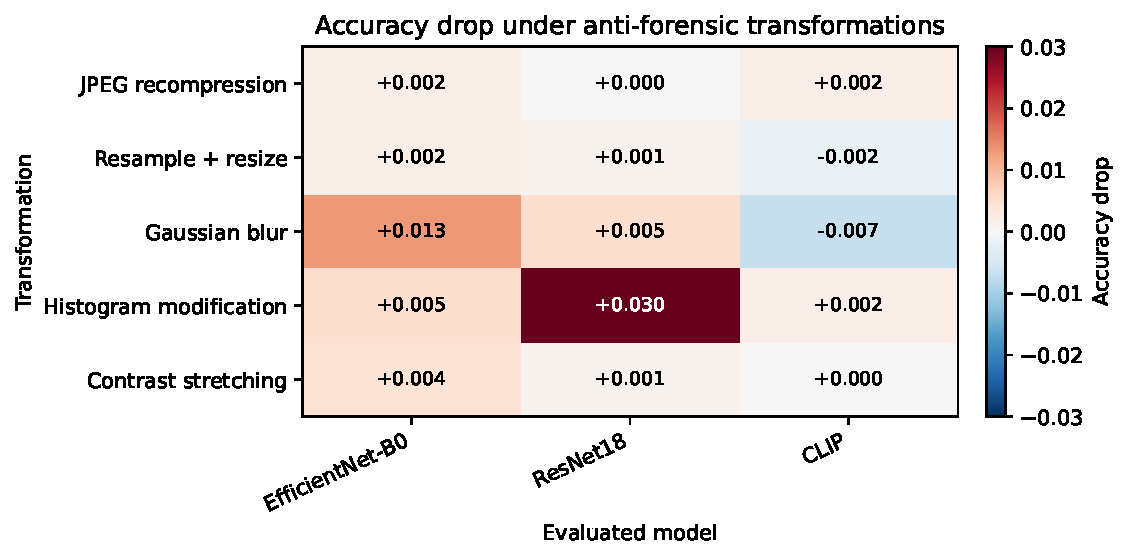
\includegraphics[width=0.88\textwidth]{images/fig_anti_forensic_accuracy_drop_heatmap.pdf}
\caption{Accuracy drop under anti-forensic transformations. The drop is defined in Section~\ref{sec:results-scope}; positive values indicate degradation with respect to the clean baseline.}
\label{fig:results-antiforensic-accuracy-drop-heatmap}
\end{figure}

The results show that the anti-forensic transformations produce overall limited
effects on the proxy models, especially when compared with the adversarial
perturbations discussed in Section~\ref{sec:results-adversarial}.
EfficientNet-B0 maintains high performance under all conditions, but is more
sensitive to \gls{gaussianblur}, with an accuracy of 0.965 and a drop of 0.013.
ResNet18, by contrast, shows the greatest degradation under
\gls{histogrammodification}, with an accuracy of 0.934 and a drop of 0.030.
\gls{clip} remains substantially stable, with very limited drops and, in some
cases, slight increases in accuracy with respect to the clean baseline.

Table~\ref{tab:results-antiforensic-operational-errors} reports additional
operational indicators for the most relevant anti-forensic conditions. These
values make it possible to distinguish the simple accuracy drop from the nature
of the induced errors, with particular attention to
\texttt{weapon}\(\rightarrow\)\texttt{non\_weapon} transitions, which represent
the most critical case in a forensic triage workflow.

\begin{table}[H]
\centering
\scriptsize
\setlength{\tabcolsep}{4pt}
\renewcommand{\arraystretch}{1.15}
\caption{Operational indicators for the most relevant anti-forensic transformations.}
\label{tab:results-antiforensic-operational-errors}
\begin{tabular}{@{}l l r r r r@{}}
\toprule
\textbf{Model} &
\textbf{Transformation} &
\textbf{Induced errors} &
\textbf{Confidence shift} &
\textbf{W\(\rightarrow\)NW} &
\textbf{NW\(\rightarrow\)W} \\
\midrule
EfficientNet-B0 & \gls{gaussianblur} & 17 & -0.0099 & 17 & 0 \\
ResNet18 & \gls{histogrammodification} & 39 & -0.0157 & 23 & 16 \\
\acrshort{clip} & \gls{histogrammodification} & 13 & -0.0037 & 6 & 7 \\
\bottomrule
\end{tabular}

\vspace{0.4em}
\footnotesize
\textit{Note.} \textit{Induced errors} indicates the number of errors introduced
with respect to correct clean predictions; \textit{Confidence shift} indicates
the mean variation in confidence with respect to the clean condition;
W\(\rightarrow\)NW indicates transitions from \texttt{weapon} to
\texttt{non\_weapon}; NW\(\rightarrow\)W indicates transitions from
\texttt{non\_weapon} to \texttt{weapon}.
\end{table}

The most critical transformation for EfficientNet-B0 is \gls{gaussianblur},
which introduces 17 errors with respect to correct clean predictions, all in the
\texttt{weapon}\(\rightarrow\)\texttt{non\_weapon} direction. For ResNet18, the
most relevant condition is \gls{histogrammodification}, which introduces 39
errors, 23 of which occur in the
\texttt{weapon}\(\rightarrow\)\texttt{non\_weapon} direction and 16 in the
opposite direction. For \gls{clip}, the effects remain more limited, although
\gls{histogrammodification} still introduces 13 errors with respect to the clean
baseline, distributed across both error directions.

From an operational perspective, these results should not be considered
negligible merely because the drops are lower than those observed under
adversarial conditions. Anti-forensic transformations are more easily
attributable to plausible conditions of image circulation, compression,
modification, and re-sharing. In a \gls{df} workflow, even a limited reduction
in performance may become relevant when it affects investigatively sensitive
content or when it combines with other sources of uncertainty, such as low image
quality, ambiguous context, or the absence of systematic human verification.

% ─────────────────────────────────────────────────────────────────────────────
\section{Adversarial Robustness}
\label{sec:results-adversarial}
% ─────────────────────────────────────────────────────────────────────────────

The adversarial evaluation measures the response of the proxy models to
perturbations designed to alter classifier
behavior~\cite{szegedy2014intriguing,goodfellow2015explaining,biggio2018wild}.
In the context of this thesis, these perturbations are not analyzed as an
autonomous objective of \gls{advml}, but as experimental stressors useful for
evaluating the operational reliability of \gls{ai}-based systems in forensic
scenarios. The main interest therefore does not concern only the ability of an
attack to reduce accuracy, but the risk that \texttt{weapon} samples are
reclassified as \texttt{non\_weapon}, generating potentially critical false
negatives in an investigative triage process.

The model-dependent attacks were generated against EfficientNet-B0. This choice
reflects a white-box scenario in which the adversary has full access to a
single target model; transferability to different architectures is therefore
evaluated empirically, rather than assumed a
priori~\cite{biggio2018wild,nowroozi2021survey,barni2018cf}. \gls{colorshift}
is instead treated as a model-agnostic adversarial-style perturbation.

Consistent with the convention defined in Section~\ref{sec:results-scope},
performance drop is interpreted as the variation with respect to the clean
baseline. In this section, negative or null values are not interpreted as
evidence of general adversarial robustness, but as effects specific to the
transferability of the perturbations generated against the target model and to
the distribution of the evaluated samples.

Table~\ref{tab:results-adversarial-robustness} reports, for each adversarial
perturbation, the perturbed accuracy and the accuracy drop with respect to the
clean baseline.

\begin{table}[H]
\centering
\scriptsize
\setlength{\tabcolsep}{3.3pt}
\renewcommand{\arraystretch}{1.15}
\caption{Perturbed accuracy and accuracy drop under adversarial perturbations.}
\label{tab:results-adversarial-robustness}
\begin{tabular}{@{}l r r r r r r@{}}
\toprule
\textbf{Perturbation} &
\textbf{\gls{clip} acc.} & \textbf{Drop} &
\textbf{EffNet acc.} & \textbf{Drop} &
\textbf{ResNet acc.} & \textbf{Drop} \\
\midrule
\gls{fgsm} & 0.914 & 0.013 & 0.575 & 0.403 & 0.918 & 0.046 \\
\gls{superdeepfool} & 0.926 & 0.001 & 0.931 & 0.047 & 0.964 & 0.000 \\
\gls{sigmazero} & 0.944 & -0.017 & 0.015 & 0.963 & 0.968 & -0.004 \\
\gls{onepixel} & 0.928 & -0.001 & 0.976 & 0.002 & 0.963 & 0.001 \\
\gls{colorshift} & 0.925 & 0.002 & 0.977 & 0.001 & 0.963 & 0.001 \\
\bottomrule
\end{tabular}

\vspace{0.4em}
\footnotesize
\textit{Note.} The drop is defined in Section~\ref{sec:results-scope};
positive values indicate degradation with respect to the clean baseline,
whereas negative values indicate a slight increase under the specific evaluated
distribution.
\end{table}

Figure~\ref{fig:results-adversarial-accuracy-drop-heatmap} visualizes the same
evaluation as a heatmap. The concentration of the highest values in the
EfficientNet-B0 column reflects the fact that the model-dependent attacks were
generated against this model.

\begin{figure}[H]
\centering
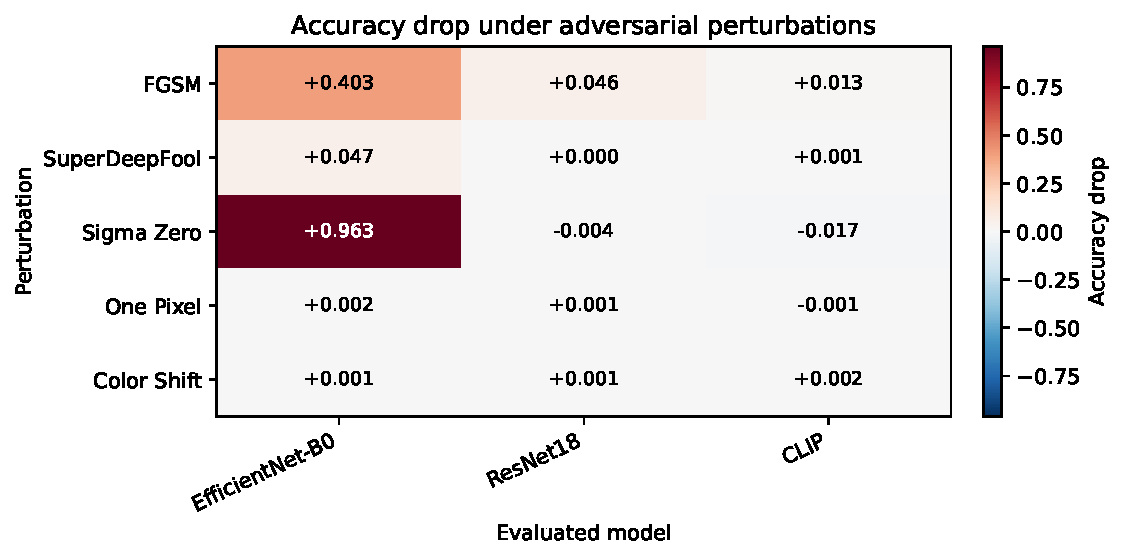
\includegraphics[width=0.88\textwidth]{images/fig_adversarial_accuracy_drop_heatmap.pdf}
\caption{Accuracy drop under adversarial perturbations. The drop is defined in Section~\ref{sec:results-scope}. The strongest degradation affects EfficientNet-B0 under \gls{sigmazero}, in the considered white-box scenario.}
\label{fig:results-adversarial-accuracy-drop-heatmap}
\end{figure}

The most critical result concerns EfficientNet-B0 under \gls{sigmazero}, where
accuracy decreases from 0.978 to 0.015, with an accuracy drop of 0.963. This
value indicates an almost complete degradation of the model's classification
capability, although limited to the white-box configuration in which the attack
is directly optimized against EfficientNet-B0 with full access to its
parameters. In operational terms, this result corresponds to behavior that is
incompatible with the unverified use of the model for the automated triage of
images containing firearm-oriented target content: the highest clean-baseline
accuracy among the proxy models does not prevent severe degradation when the
model is exposed to perturbations optimized against it.

\gls{fgsm}, also generated against EfficientNet-B0, produces a relevant
degradation, reducing accuracy to 0.575 and yielding an accuracy drop of 0.403.
\gls{superdeepfool} instead produces a more limited effect on the same model,
with an accuracy of 0.931 and a drop of 0.047. \gls{onepixel} and
\gls{colorshift} produce marginal variations on EfficientNet-B0, equal to
0.002 and 0.001, respectively.

The comparison with ResNet18 and \gls{clip} shows that the transfer of attacks
generated against EfficientNet-B0 does not produce equivalent degradation on
the other models. ResNet18 undergoes the largest drop under \gls{fgsm}, equal
to 0.046, while remaining substantially stable with respect to
\gls{superdeepfool}, \gls{onepixel}, \gls{sigmazero}, and \gls{colorshift}.
\gls{clip} shows even more limited variations, with the maximum degradation
equal to 0.013 under \gls{fgsm}. In some cases, such as \gls{sigmazero}, the
perturbed accuracy of \gls{clip} and ResNet18 is slightly higher than the
respective clean baseline; this effect is interpreted as an oscillation
specific to the evaluated distribution and not as evidence of general
robustness.

Table~\ref{tab:results-adversarial-operational-errors} reports additional
operational indicators for the most relevant adversarial conditions. These
values make it possible to distinguish the accuracy drop from the direction of
the induced errors, with particular attention to
\texttt{weapon}\(\rightarrow\)\texttt{non\_weapon} transitions.

\begin{table}[H]
\centering
\scriptsize
\setlength{\tabcolsep}{3.5pt}
\renewcommand{\arraystretch}{1.15}
\caption{Operational indicators for the most relevant adversarial perturbations.}
\label{tab:results-adversarial-operational-errors}
\begin{tabular}{@{}l l r r r r r@{}}
\toprule
\textbf{Model} &
\textbf{Perturbation} &
\textbf{Induced errors} &
\textbf{ASR} &
\textbf{Confidence shift} &
\textbf{W\(\rightarrow\)NW} &
\textbf{NW\(\rightarrow\)W} \\
\midrule
EfficientNet-B0 & \gls{sigmazero} & 963 & 0.9847 & -0.2578 & 489 & 474 \\
EfficientNet-B0 & \gls{fgsm} & 406 & 0.4151 & -0.1246 & 321 & 85 \\
EfficientNet-B0 & \gls{superdeepfool} & 47 & 0.0481 & -0.3063 & 0 & 47 \\
ResNet18 & \gls{fgsm} & 47 & 0.0488 & -0.0230 & 27 & 20 \\
\acrshort{clip} & \gls{fgsm} & 23 & 0.0248 & -0.0043 & 8 & 15 \\
\bottomrule
\end{tabular}

\vspace{0.4em}
\footnotesize
\textit{Note.} \textit{Induced errors} indicates the number of errors introduced
with respect to correct clean predictions; \textit{ASR} indicates the attack
success rate computed with respect to samples correctly classified under clean
conditions; \textit{Confidence shift} indicates the mean variation in
confidence with respect to the clean condition; W\(\rightarrow\)NW indicates
transitions from \texttt{weapon} to \texttt{non\_weapon}; NW\(\rightarrow\)W
indicates transitions from \texttt{non\_weapon} to \texttt{weapon}.
\end{table}

The analysis of the induced errors confirms the operational criticality of the
EfficientNet-B0 scenario under \gls{sigmazero}: 963 errors are introduced with
respect to correct clean predictions, including 489
\texttt{weapon}\(\rightarrow\)\texttt{non\_weapon} transitions. This aspect is
more relevant than accuracy alone, because it directly describes the risk of
failing to flag content belonging to the investigatively relevant class.
\gls{fgsm} also produces a significant effect on EfficientNet-B0, with 406
induced errors and 321 \texttt{weapon}\(\rightarrow\)\texttt{non\_weapon}
transitions. For ResNet18 and \gls{clip}, the transferred effects are more
limited, but not absent.

From a forensic perspective, the vulnerability of EfficientNet-B0 to
perturbations such as \gls{sigmazero} and \gls{fgsm} highlights a significant
operational risk: a system that appears highly accurate under clean conditions
may degrade drastically when exposed to deliberately manipulated inputs. This
reinforces the need not to interpret the output of an \gls{ai}-based classifier
as autonomous evidence, but as triage support that must be subjected to
verification, traceability, and evaluation within the overall investigative
context.


% ─────────────────────────────────────────────────────────────────────────────
\section{Forensic Evaluation Bundle Composition and Black-Box Readiness}
\label{sec:results-bundle}
% ─────────────────────────────────────────────────────────────────────────────

The forensic evaluation bundle constitutes the connection layer between the
controlled experimental evaluation of the proxy models and the subsequent
black-box evaluation of the selected commercial software systems. The bundle is
designed to provide the evaluated software with a blind and semantically
neutral input, while separately preserving the information required for
matching, export normalization, and result
auditing~\cite{casey2011digital,nist2006guide,iso27041,iso27042,swgde2014validation}.

Unlike the general composition of the experimental corpus reported in
Section~\ref{sec:results-scope},
Table~\ref{tab:results-bundle-operational-layout} describes the bundle from an
operational perspective, distinguishing among the content submitted to the
software systems, blind naming, and the role of metadata in the audit phase.
The total consists of 11\,500 files, including 1\,000 clean samples,
500 \gls{ood} samples, 5\,000 adversarial samples, and 5\,000 anti-forensic
samples.

\begin{table}[H]
\centering
\scriptsize
\renewcommand{\arraystretch}{1.15}
\setlength{\tabcolsep}{4pt}
\caption{Operational view of the forensic evaluation bundle for black-box evaluation.}
\label{tab:results-bundle-operational-layout}
\begin{tabularx}{\textwidth}{@{}l r l X@{}}
\toprule
\textbf{Component} &
\textbf{Files} &
\textbf{Blind input} &
\textbf{Role of metadata} \\
\midrule

Clean &
1\,000 &
\texttt{bundle\_*.jpg} &
Preserves the correspondence with the original binary subset and with the
\texttt{weapon}/\texttt{non\_weapon} label. \\

\gls{ood} &
500 &
\texttt{bundle\_*.jpg} &
Preserves the distinction between out-of-distribution samples and the nominal
binary task. \\

Adversarial &
5\,000 &
\texttt{bundle\_*.jpg} &
Records the attack family, perturbation name, target model, and source image. \\

Anti-forensic &
5\,000 &
\texttt{bundle\_*.jpg} &
Records the applied transformation, source image, and mapping to the
corresponding clean sample. \\

\midrule
\textbf{Total} &
\textbf{11\,500} &
\texttt{bundle\_*.jpg} &
Enables matching, post-export normalization, and hash-based auditing. \\
\bottomrule
\end{tabularx}
\end{table}

The bundle construction follows two complementary views. The first is a blind
directory intended for the evaluated software, in which files are renamed with
neutral identifiers such as \texttt{bundle\_000001.jpg}. The second is a
structured audit view, reserved for the researcher, in which the semantic and
experimental information required for verification is preserved. For black-box
evaluation, the software systems must import only the directory:

\begin{center}
\codepath{datasets/forensic_evaluation_bundle/blind_tool_input/files}
\end{center}

and must not import either the \codepath{metadata/} directory or the
\codepath{structured_audit_view/} directory. This separation reduces the risk
of bias induced by file names, paths, classes, attack names, or split
structure.

The bundle preserves traceability through separate manifests containing, for
each file, the bundle identifier, blind name, sample type, perturbation family
and name, fold, final label, source dataset, original image identifier, source
path, blind path, structured path, \gls{sha256} hash, \gls{md5} hash, file
size, and extension. This structure makes it possible to connect each output
exported by a software system to the corresponding experimental artifact
without exposing the ground truth to the software during the import phase.

The consistency checks verified that the bundle identifiers are unique, that
the actual \gls{sha256} hashes are unique, that the computed hashes match those
reported in the manifest when available, that the blind paths are semantically
neutral, and that the experimental metadata are separated from the operational
input submitted to the software systems. These checks are essential to make the
bundle suitable for black-box evaluation, since they make it possible to
distinguish among classification errors, unprocessed files, uncategorized
outputs, limitations of the export format, and matching
problems~\cite{iso27041,iso27042,iso27043,swgde2014validation}.

In summary, the forensic evaluation bundle makes it possible to move from a
fully controlled proxy evaluation to an evaluation closer to the operational
context of selected black-box software systems. Its function is not merely
organizational, but methodological: it preserves the reproducibility of the
experiment and reduces the exposure of the evaluated software to unnecessary
semantic information. At the same time, it enables post-export normalization
based on verifiable identifiers and hashes, which is a necessary condition for
distinguishing genuine classification errors from artifacts of the export
process or limitations of the operational mapping.

A specific control on residual embedded metadata in the blind view of the
bundle is discussed in
Section~\ref{subsec:results-embedded-metadata-sensitivity}, after the
presentation of the normalized outputs of the selected software systems, since
its interpretation requires comparison with the observed black-box results.













% ─────────────────────────────────────────────────────────────────────────────
\section{Commercial Forensic Tools Evaluation}
\label{sec:results-commercial}
% ─────────────────────────────────────────────────────────────────────────────

The evaluation of commercial tools represents the black-box level of the
experimental pipeline. Unlike the proxy models analyzed in the previous
sections, these tools do not provide access to the model architecture, training
dataset, decision thresholds, internal preprocessing, or complete
classification logic. The evaluation is therefore based exclusively on the
observable outputs produced by the tools, such as assigned tags, exported
categories, retrieval results, and semantic bookmarks, as well as on the
matching between the files of the forensic evaluation bundle and the
experimental ground truth.

The commercial comparison includes four final tools:
\gls{magnetaxiomtool}/\gls{magnetai}, \gls{excirefoto2025},
\gls{cellebriteinseyets}, and \gls{griffeye}/\gls{t3kcore}. Since
\gls{excirefoto2025} is evaluated through three operational configurations of
the \texttt{Distance limit} parameter, the metric comparison produces six
normalized commercial profiles: \gls{magnetaxiomtool}/\gls{magnetai},
\gls{excirefoto2025} \texttt{D20}, \gls{excirefoto2025} \texttt{D50},
\gls{excirefoto2025} \texttt{D80}, \gls{cellebriteinseyets}, and
\gls{griffeye}/\gls{t3kcore}.

The commercial tools are not treated as homogeneous classifiers. \gls{magnetai}
exposes operational image categorization outputs; \gls{excirefoto2025} operates
as a semantic retrieval engine; \gls{cellebriteinseyets} produces media analysis
outputs exported from the Cellebrite environment; and
\gls{griffeye}/\gls{t3kcore} produces automatic semantic bookmarks. The
comparison is therefore operational and black-box: each output is mapped to the
\texttt{weapon}/\texttt{non\_weapon} task through explicit and documented
normalization rules.

The adversarial perturbations included in the bundle must not be interpreted as
white-box attacks optimized against the proprietary commercial tools. They are
artifacts generated within the controlled proxy-model protocol and are used here
to observe, in black-box mode, the operational sensitivity of commercial tools
to manipulated inputs. Moreover, the aggregate metrics for commercial tools are
\emph{bundle-weighted}: they describe behavior within the forensic evaluation
bundle, whose composition is intentionally oriented toward robustness analysis,
and not an absolute estimate of the overall quality of the product.

To prevent the tools from using semantic information derived from file names,
paths, or folder structure, the evaluation was conducted using the blind view of
the forensic evaluation bundle. The files were imported with neutral names such
as \texttt{bundle\_*.jpg}, while information related to class, source, fold,
attack, transformation, hash, and ground truth was kept separate in the audit
manifests. After processing, the exported outputs were normalized and mapped
back to the original samples through bundle identifiers and
\gls{sha256}/\gls{md5} hashes. This setting makes it possible to distinguish
among correctly flagged images, unflagged images, false negatives on the
\texttt{weapon} class, false positives on the \texttt{non\_weapon} class,
non-interpretable outputs, and behavior on \gls{ood} samples.

Table~\ref{tab:results-commercial-overview} reports a bundle-weighted summary
of the metrics for the commercial systems and operational configurations
considered. For all commercial profiles, normalization produced complete
matching against the forensic evaluation bundle (11\,500/11\,500 files), with
no unmapped rows or non-interpretable outputs. For \gls{excirefoto2025}, the
three rows correspond to the \texttt{D20}, \texttt{D50}, and \texttt{D80}
configurations of the \texttt{Distance limit} parameter. The \texttt{D50}
configuration is used as the main reference in the comparative discussion,
because it represents an intermediate compromise between the restrictive and
permissive configurations.

\begin{table}[H]
\centering
\scriptsize
\renewcommand{\arraystretch}{1.15}
\setlength{\tabcolsep}{2.6pt}
\caption{Bundle-weighted summary of the black-box evaluation of commercial systems.}
\label{tab:results-commercial-overview}
\begin{tabular}{@{}l r r r r r r r r@{}}
\toprule
\textbf{System} &
\textbf{Matched} &
\textbf{Clean FNR} &
\textbf{Acc.} &
\textbf{Bal.} &
\textbf{R\textsubscript{w}} &
\textbf{\acrshort{fnr}} &
\textbf{\acrshort{fpr}} &
\textbf{OOD W-rate} \\
\midrule
\gls{magnetaxiomtool}/\gls{magnetai}
& 11\,500 & 0.070 & 0.933 & 0.933 & 0.901 & 0.099 & 0.035 & 0.360 \\

\gls{excirefoto2025} \texttt{D20}
& 11\,500 & 0.120 & 0.911 & 0.911 & 0.857 & 0.143 & 0.036 & 0.238 \\

\gls{excirefoto2025} \texttt{D50}
& 11\,500 & 0.042 & 0.925 & 0.925 & 0.949 & 0.051 & 0.099 & 0.340 \\

\gls{excirefoto2025} \texttt{D80}
& 11\,500 & 0.014 & 0.887 & 0.887 & 0.981 & 0.019 & 0.207 & 0.522 \\

\gls{cellebriteinseyets}
& 11\,500 & 0.032 & 0.958 & 0.958 & 0.958 & 0.042 & 0.042 & 0.292 \\

\gls{griffeye}/\gls{t3kcore}
& 11\,500 & 0.036 & 0.972 & 0.972 & 0.951 & 0.049 & 0.007 & 0.260 \\

\bottomrule
\end{tabular}

\vspace{0.4em}
\footnotesize
\textit{Note.} \textit{Matched} indicates the number of files in the forensic
evaluation bundle mapped to a normalized output. \textit{Clean FNR} indicates
the false negative rate observed on the unperturbed baseline. \textit{Acc.}
indicates accuracy on the interpretable binary task; \textit{Bal.} indicates
balanced accuracy; \(R_w\) indicates recall for the \texttt{weapon} class;
\gls{fnr} and \gls{fpr} indicate false negative rate and false positive rate on
the overall binary bundle, respectively; \textit{OOD W-rate} indicates the
proportion of \gls{ood} samples operationally mapped to the \texttt{weapon}
class. Binary metrics are computed on \texttt{weapon}/\texttt{non\_weapon}
samples; \gls{ood} samples are analyzed separately. The values are
bundle-weighted and reflect the experimental composition of the bundle, not a
general product validation.
\end{table}

\begin{figure}[H]
\centering
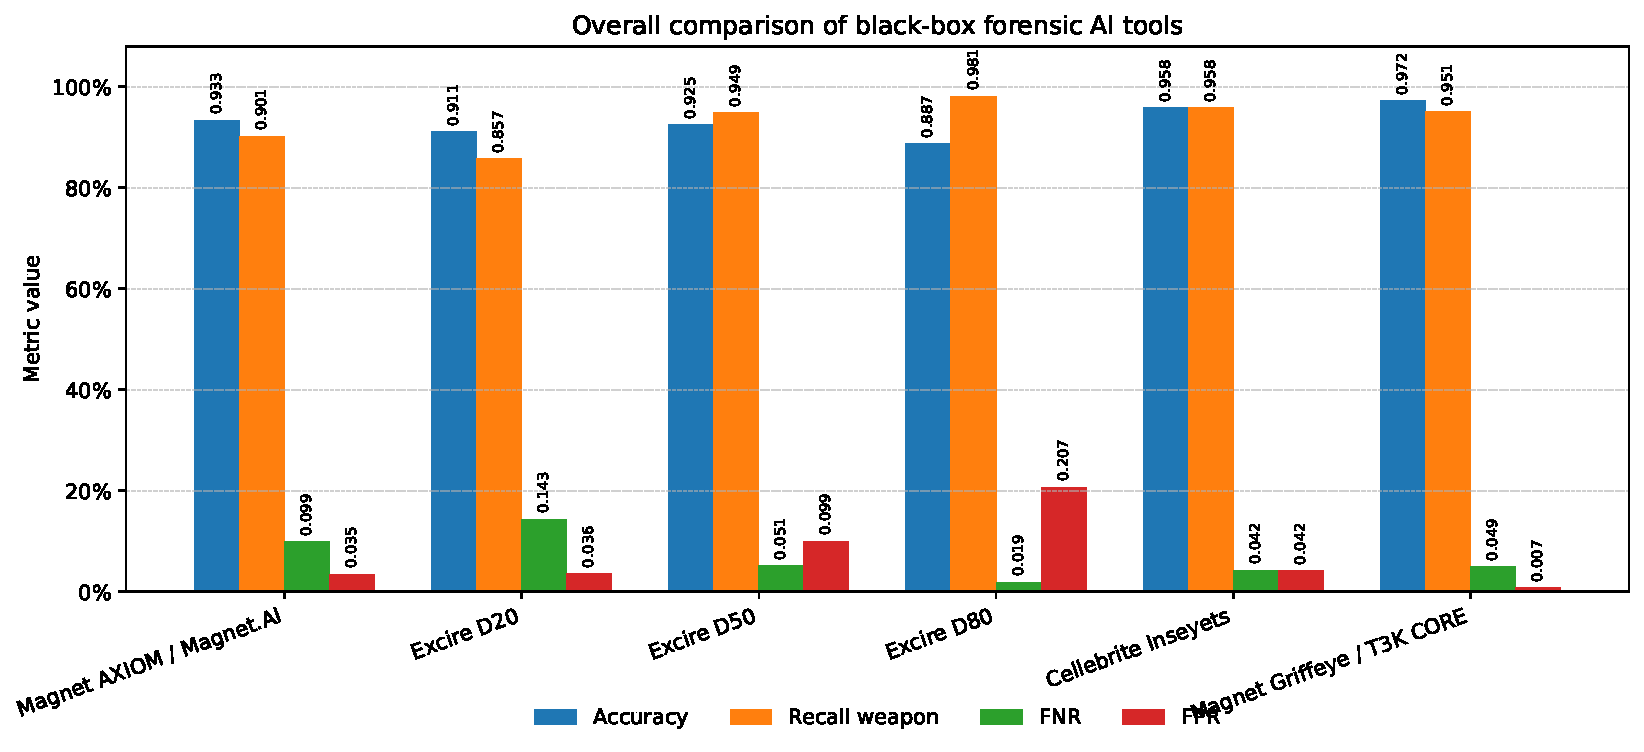
\includegraphics[width=0.95\textwidth]{images/fig_forensic_tools_global_metrics_comparison.pdf}
\caption{Global comparison of the aggregate metrics of the commercial black-box tools on the forensic evaluation bundle. The plot compares accuracy, balanced accuracy, \texttt{weapon} recall, FNR, FPR, and OOD weapon flag rate after output normalization.}
\label{fig:results-forensic-tools-global-comparison}
\end{figure}

Table~\ref{tab:results-commercial-overview} and
Figure~\ref{fig:results-forensic-tools-global-comparison} must be interpreted
with caution. The metrics do not describe the internal accuracy of the
commercial systems in an absolute sense, but the behavior observed after output
normalization in the operational \texttt{weapon}/\texttt{non\_weapon} task. In
particular, the case of \gls{excirefoto2025} clearly shows the effect of the
retrieval threshold: \texttt{D20} reduces the false positive rate and the weapon
flag rate on \gls{ood} samples, but increases false negatives; \texttt{D80}
maximizes recall on the \texttt{weapon} class, but markedly increases false
positives and \texttt{weapon} flags on \gls{ood} samples. \texttt{D50}
therefore represents an intermediate configuration, useful for the operational
comparison with \gls{magnetai}, \gls{cellebriteinseyets}, and
\gls{griffeye}/\gls{t3kcore}.

\begin{figure}[H]
\centering
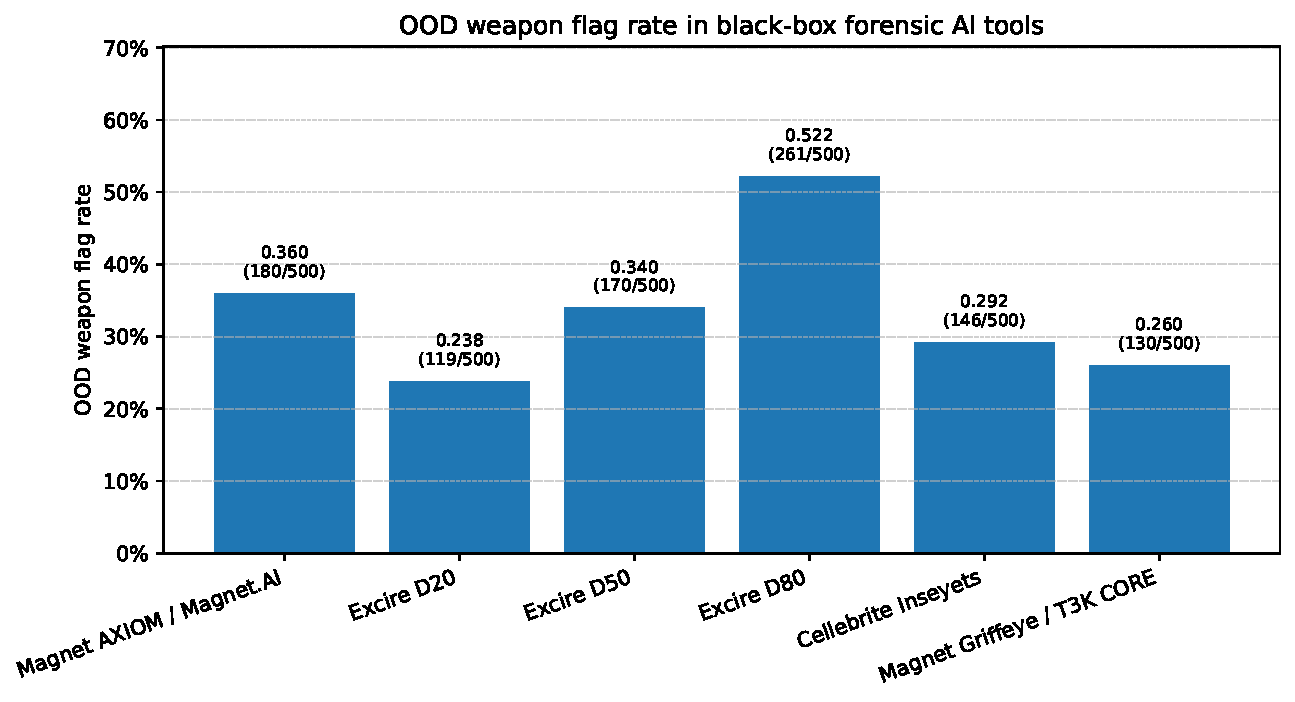
\includegraphics[width=0.90\textwidth]{images/fig_forensic_tools_ood_weapon_flag_rate.pdf}
\caption{Weapon flag rate of the commercial black-box tools on \gls{ood} samples.}
\label{fig:results-forensic-tools-ood-weapon-flag-rate}
\end{figure}

Figure~\ref{fig:results-forensic-tools-ood-weapon-flag-rate} shows that even
commercial tools with good performance on the binary task exhibit a non-zero
rate of absorption of \gls{ood} samples into the operational \texttt{weapon}
class. This behavior is particularly relevant for forensic triage, since it may
increase the human review workload and assign investigative priority to content
that is semantically ambiguous or external to the main task.

Overall, this section introduces the black-box level of the evaluation. The
following subsections analyze the results of
\gls{magnetaxiomtool}/\gls{magnetai}, \gls{excirefoto2025},
\gls{cellebriteinseyets}, and \gls{griffeye}/\gls{t3kcore} separately,
distinguishing clean performance, behavior on perturbed inputs, false negative
risk on the \texttt{weapon} class, and weapon flag rate on \gls{ood} samples.





% ─────────────────────────────────────────────────────────────────────────────
\subsection{Magnet AXIOM / Magnet.AI Results}
\label{subsec:results-magnet}
% ─────────────────────────────────────────────────────────────────────────────

The evaluation of \gls{magnetaxiomtool}/\gls{magnetai} constitutes the first
consolidated commercial black-box result of the pipeline. The outputs produced
by the tool were normalized by mapping the \texttt{Possible weapons} tag as an
operational positive prediction for the \texttt{weapon} class; the absence of
this tag was instead mapped to the negative prediction
\texttt{non\_weapon}. This recoding makes it possible to compare the observable
output of the tool with the experimental ground truth of the forensic evaluation
bundle, without assuming access to the internal decision logic of the
proprietary module.

As indicated in Section~\ref{sec:results-commercial}, matching between the
commercial export and the forensic evaluation bundle is complete for all
evaluated profiles. For \gls{magnetai}, the binary metrics are therefore
computed on the 11\,000 images belonging to the operational classes
\texttt{weapon} and \texttt{non\_weapon}; the 500 \gls{ood} images are analyzed
separately through the weapon flag rate.

Table~\ref{tab:results-magnet-global-metrics} reports the overall metrics of
\gls{magnetai} on the binary \texttt{weapon}/\texttt{non\_weapon} task. The tool
achieves an accuracy of 0.933 and a precision of 0.963 on the \texttt{weapon}
class. However, recall on the \texttt{weapon} class is 0.901, with a \gls{fnr}
of 0.099: 542 images belonging to the \texttt{weapon} class were not flagged as
\texttt{Possible weapons}.

\begin{table}[H]
\centering
\caption{Overall performance of \gls{magnetai} on the binary \texttt{weapon}/\texttt{non\_weapon} task.}
\label{tab:results-magnet-global-metrics}
\small
\begin{tabular}{lr}
\toprule
\textbf{Metric} & \textbf{Value} \\
\midrule
Accuracy & 0.933 \\
Balanced accuracy & 0.933 \\
Precision \texttt{weapon} & 0.963 \\
Recall \texttt{weapon} & 0.901 \\
F1 \texttt{weapon} & 0.931 \\
False negative rate & 0.099 \\
False positive rate & 0.035 \\
True positives & 4\,958 \\
True negatives & 5\,309 \\
False positives & 191 \\
False negatives & 542 \\
\bottomrule
\end{tabular}

\vspace{0.4em}
\footnotesize
\textit{Note.} The metrics are computed on the 11\,000 images belonging to the
binary \texttt{weapon}/\texttt{non\_weapon} task. The aggregate value does not
correspond to the arithmetic mean between clean and perturbed conditions,
because the bundle includes 1\,000 clean images and 10\,000 perturbed images.
\end{table}

The note reported in Table~\ref{tab:results-magnet-global-metrics} highlights
that the aggregate value is influenced by the composition of the bundle, in
which perturbed images are numerically predominant with respect to clean
samples. The overall metrics must therefore be read together with the
disaggregation by experimental condition reported in
Table~\ref{tab:results-magnet-condition-metrics}.

\begin{table}[H]
\centering
\caption{Behavior of \gls{magnetai} by experimental condition.}
\label{tab:results-magnet-condition-metrics}
\small
\begin{tabularx}{\textwidth}{@{}l r r r r X@{}}
\toprule
\textbf{Condition} &
\textbf{Accuracy} &
\textbf{Recall weapon} &
\textbf{\gls{fnr}} &
\textbf{\gls{fpr}} &
\textbf{Operational note} \\
\midrule

Clean &
0.950 &
0.930 &
0.070 &
0.030 &
Commercial baseline on 1\,000 unperturbed images. \\

Perturbed &
0.932 &
0.899 &
0.101 &
0.035 &
Values computed on 10\,000 perturbed images: 5\,000 adversarial and 5\,000
anti-forensic. The main degradation concerns the increase in false negatives on
the \texttt{weapon} class. \\

Adversarial &
0.923 &
0.884 &
0.116 &
0.038 &
Aggregate performance across the five adversarial perturbations considered. \\

Anti-forensic &
0.940 &
0.913 &
0.087 &
0.032 &
Aggregate performance across the five anti-forensic transformations considered. \\

\gls{ood} &
-- &
-- &
-- &
-- &
Weapon flag rate equal to 0.360: 180 \gls{ood} images out of 500 were flagged
as \texttt{Possible weapons}. Standard binary metrics are not applicable. \\

\bottomrule
\end{tabularx}
\end{table}

The disaggregation by condition shows that adversarial attacks produce a more
pronounced impact than anti-forensic transformations. The aggregate \gls{fnr}
under adversarial conditions is 0.116, compared with 0.087 for anti-forensic
transformations. This result indicates that, in the case of \gls{magnetai},
perturbations designed to interfere with classifier behavior produce a more
substantial increase in false negatives than realistic image degradation or
manipulation transformations.

The behavior on \gls{ood} images is relevant for the triage workflow.
Out-of-distribution images do not belong to the binary
\texttt{weapon}/\texttt{non\_weapon} task and therefore should not be
interpreted as classical classification errors. However, the fact that 180
\gls{ood} images out of 500 were flagged as \texttt{Possible weapons} indicates
that the automatic module may assign investigative relevance to content that is
semantically ambiguous or does not belong to the expected distribution.

Unlike the proxy models, \gls{magnetai} does not export numerical confidence
values associated with individual predictions. The observable classification is
based exclusively on the presence or absence of the \texttt{Possible weapons}
tag, without a quantitative indication of the degree of certainty. This
characteristic prevents direct comparison with the confidence distributions of
the proxy models and constitutes an operational limitation for the interpretive
traceability of the output.

Table~\ref{tab:results-magnet-attack-metrics} reports the behavior of
\gls{magnetai} with respect to all perturbations considered in the forensic
evaluation bundle. The condition-level detail shows an increase in false
negatives especially under \gls{fgsm}, with an accuracy of 0.867, recall on the
\texttt{weapon} class equal to 0.808, and a \gls{fnr} of 0.192. Among the
anti-forensic transformations, \gls{gaussianblur} produces the highest
\gls{fnr}, equal to 0.120.

\begin{table}[H]
\centering
\caption{Performance of \gls{magnetai} under adversarial and anti-forensic conditions.}
\label{tab:results-magnet-attack-metrics}
\scriptsize
\renewcommand{\arraystretch}{1.12}
\setlength{\tabcolsep}{4pt}
\begin{tabular}{@{}l l r r r r r r@{}}
\toprule
\textbf{Family} &
\textbf{Condition} &
\textbf{Accuracy} &
\textbf{Recall} &
\textbf{\gls{fnr}} &
\textbf{\gls{fpr}} &
\textbf{FN} &
\textbf{FP} \\
\midrule

Adversarial &
\gls{colorshift} &
0.951 &
0.934 &
0.066 &
0.032 &
33 &
16 \\

Adversarial &
\gls{fgsm} &
0.867 &
0.808 &
0.192 &
0.074 &
96 &
37 \\

Adversarial &
\gls{onepixel} &
0.950 &
0.930 &
0.070 &
0.030 &
35 &
15 \\

Adversarial &
\gls{sigmazero} &
0.916 &
0.856 &
0.144 &
0.024 &
72 &
12 \\

Adversarial &
\gls{superdeepfool} &
0.932 &
0.894 &
0.106 &
0.030 &
53 &
15 \\

\midrule

Anti-forensic &
\gls{contraststretching} &
0.951 &
0.930 &
0.070 &
0.028 &
35 &
14 \\

Anti-forensic &
\gls{gaussianblur} &
0.927 &
0.880 &
0.120 &
0.026 &
60 &
13 \\

Anti-forensic &
\gls{histogrammodification} &
0.936 &
0.920 &
0.080 &
0.048 &
40 &
24 \\

Anti-forensic &
\gls{jpegrecompression} &
0.944 &
0.928 &
0.072 &
0.040 &
36 &
20 \\

Anti-forensic &
\gls{resampleresize} &
0.943 &
0.906 &
0.094 &
0.020 &
47 &
10 \\

\bottomrule
\end{tabular}
\end{table}

Overall, \gls{magnetai} shows good accuracy under clean conditions, equal to
0.950, with a low \gls{fpr} of 0.030. However, the \gls{fnr} of 0.070 indicates
that even in the absence of perturbations a non-negligible proportion of
\texttt{weapon} images is not flagged. This value increases in the presence of
some adversarial perturbations, with a relevant operational impact for triage.
From this perspective, the most important datum is not accuracy reduction alone,
but the increase in false negatives: in a triage scenario, a \texttt{weapon}
image not flagged by the automatic module may receive lower priority for human
review.

These results must be interpreted as indicators of operational reliability, not
as a measure of the internal algorithmic robustness of \gls{magnetai}, which
remains non-inspectable. The tool maintains good overall performance and high
precision on the \texttt{weapon} class, but produces false negatives under both
clean and perturbed conditions and flags a non-negligible proportion of
\gls{ood} images as \texttt{Possible weapons}. These findings support the need
to treat automatic output as an aid to triage and not as a conclusive or
self-sufficient decision.


% ─────────────────────────────────────────────────────────────────────────────
\subsection{Excire Foto 2025 Results and Sensitivity Analysis}
\label{subsec:results-excire}
% ─────────────────────────────────────────────────────────────────────────────

The evaluation of \gls{excirefoto2025} requires specific interpretive caution.
The software is not treated as a product developed exclusively for forensic
purposes, nor as a native classifier for the binary
\texttt{weapon}/\texttt{non\_weapon} distinction. In the experimental protocol,
it is evaluated as a black-box semantic retrieval system equipped with
\gls{ai}-based functionalities. The operational prediction is therefore derived
from the presence or absence of a sample among the results retrieved by the
configured semantic search. This recoding enables a quantitative evaluation
against the experimental ground truth, but it must not be interpreted as access
to the internal classification logic of the system.

To evaluate the sensitivity of the operational behavior to the retrieval
threshold, three configurations of the \texttt{Distance limit} parameter were
considered: \texttt{D20}, \texttt{D50}, and \texttt{D80}. The \texttt{D20}
configuration represents a restrictive setting, oriented toward reducing false
positives and semantically weak retrievals; \texttt{D50} constitutes the
intermediate configuration of the sensitivity analysis; \texttt{D80} instead
represents a permissive setting, oriented toward maximizing recall but exposed
to a substantial increase in false positives and in the weapon flag rate on
\gls{ood} samples.

\begin{table}[H]
\centering
\scriptsize
\renewcommand{\arraystretch}{1.15}
\setlength{\tabcolsep}{4pt}
\caption{Sensitivity analysis of \gls{excirefoto2025} with respect to the \texttt{Distance limit} parameter.}
\label{tab:results-excire-sensitivity}
\begin{tabularx}{0.95\textwidth}{@{}l r r r r r X@{}}
\toprule
\textbf{Setting} &
\textbf{Clean Acc.} &
\textbf{Recall} &
\textbf{\gls{fnr}} &
\textbf{\gls{fpr}} &
\textbf{OOD W-rate} &
\textbf{Operational profile} \\
\midrule

\texttt{D20} &
0.927 &
0.880 &
0.120 &
0.026 &
0.238 &
Restrictive: low operational noise and lower \gls{ood} absorption, but higher
risk of false negatives. \\

\texttt{D50} &
0.944 &
0.958 &
0.042 &
0.070 &
0.340 &
Intermediate: more balanced compromise in the experimental context considered. \\

\texttt{D80} &
0.915 &
0.986 &
0.014 &
0.156 &
0.522 &
Permissive: very high recall, but marked increase in false positives and
\gls{ood} flags. \\

\bottomrule
\end{tabularx}
\end{table}

The comparison among the three configurations shows that the
\texttt{Distance limit} parameter does not act as a merely technical variable,
but as an operational threshold that modifies the risk profile of the system.
\texttt{D20} is more conservative and reduces the review workload arising from
false positives, but may fail to retrieve relevant \texttt{weapon} content.
\texttt{D50} represents, in the experimental context considered, the most
balanced configuration for triage, since it maintains high recall on the
\texttt{weapon} class without producing the level of noise observed under
\texttt{D80}. The latter strongly reduces false negatives, but substantially
increases false positives and maps more than half of the \gls{ood} inputs to
the \texttt{weapon} class.

\begin{table}[H]
\centering
\caption{Aggregate performance of \gls{excirefoto2025} under perturbed conditions.}
\label{tab:results-excire-perturbed-summary}
\small
\begin{tabular}{l l r r r r}
\toprule
\textbf{Setting} &
\textbf{Condition} &
\textbf{Accuracy} &
\textbf{Recall weapon} &
\textbf{\gls{fnr}} &
\textbf{\gls{fpr}} \\
\midrule

\texttt{D20} & Anti-forensic & 0.927 & 0.875 & 0.125 & 0.022 \\
\texttt{D50} & Anti-forensic & 0.941 & 0.957 & 0.043 & 0.074 \\
\texttt{D80} & Anti-forensic & 0.908 & 0.984 & 0.016 & 0.169 \\

\midrule

\texttt{D20} & Adversarial & 0.892 & 0.834 & 0.166 & 0.051 \\
\texttt{D50} & Adversarial & 0.904 & 0.938 & 0.062 & 0.130 \\
\texttt{D80} & Adversarial & 0.861 & 0.977 & 0.023 & 0.256 \\

\bottomrule
\end{tabular}
\end{table}

The aggregate results under perturbed conditions show that, for
\gls{excirefoto2025}, anti-forensic transformations produce a more limited
impact than adversarial perturbations. However, in this case as well, the
operational profile changes substantially as the threshold varies:
\texttt{D20} maintains the lowest \gls{fpr} but presents the highest \gls{fnr},
\texttt{D80} almost completely reduces false negatives but increases
operational noise, whereas \texttt{D50} maintains an intermediate compromise
between recall and selectivity.

Table~\ref{tab:results-excire-d50-attack-metrics} reports the detailed results
for the \texttt{D50} configuration, which is used as the main reference for the
operational comparison. This choice does not imply that \texttt{D50} is optimal
in an absolute sense, but makes it possible to analyze an intermediate
configuration between the restrictive and permissive profiles.

\begin{table}[H]
\centering
\caption{Performance of \gls{excirefoto2025} \texttt{D50} under adversarial and anti-forensic conditions.}
\label{tab:results-excire-d50-attack-metrics}
\scriptsize
\renewcommand{\arraystretch}{1.12}
\setlength{\tabcolsep}{4pt}
\begin{tabular}{@{}l l r r r r r r@{}}
\toprule
\textbf{Family} &
\textbf{Condition} &
\textbf{Accuracy} &
\textbf{Recall} &
\textbf{\gls{fnr}} &
\textbf{\gls{fpr}} &
\textbf{FN} &
\textbf{FP} \\
\midrule

Adversarial &
\gls{colorshift} &
0.949 &
0.966 &
0.034 &
0.068 &
17 &
34 \\

Adversarial &
\gls{fgsm} &
0.926 &
0.890 &
0.110 &
0.038 &
55 &
19 \\

Adversarial &
\gls{onepixel} &
0.946 &
0.964 &
0.036 &
0.072 &
18 &
36 \\

Adversarial &
\gls{sigmazero} &
0.742 &
0.926 &
0.074 &
0.442 &
37 &
221 \\

Adversarial &
\gls{superdeepfool} &
0.956 &
0.944 &
0.056 &
0.032 &
28 &
16 \\

\midrule

Anti-forensic &
\gls{contraststretching} &
0.941 &
0.952 &
0.048 &
0.070 &
24 &
35 \\

Anti-forensic &
\gls{gaussianblur} &
0.941 &
0.960 &
0.040 &
0.078 &
20 &
39 \\

Anti-forensic &
\gls{histogrammodification} &
0.932 &
0.952 &
0.048 &
0.088 &
24 &
44 \\

Anti-forensic &
\gls{jpegrecompression} &
0.946 &
0.958 &
0.042 &
0.066 &
21 &
33 \\

Anti-forensic &
\gls{resampleresize} &
0.947 &
0.964 &
0.036 &
0.070 &
18 &
35 \\

\bottomrule
\end{tabular}
\end{table}

A particularly relevant case is represented by \gls{sigmazero}. Unlike a simple
evasion dynamic, in which the main effect would be the increase in false
negatives on the \texttt{weapon} class, \gls{excirefoto2025} shows, under the
\texttt{D50} and \texttt{D80} configurations, a behavior of semantic
over-triggering. Under these conditions, the system continues to retrieve many
\texttt{weapon} images, but substantially increases the proportion of
\texttt{non\_weapon} images erroneously retrieved as relevant.

\begin{table}[H]
\centering
\caption{Behavior of \gls{excirefoto2025} on the \gls{sigmazero} perturbation.}
\label{tab:results-excire-sigma-zero}
\small
\begin{tabular}{l r r r r r r}
\toprule
\textbf{Setting} &
\textbf{Accuracy} &
\textbf{Recall} &
\textbf{\gls{fnr}} &
\textbf{\gls{fpr}} &
\textbf{FN} &
\textbf{FP} \\
\midrule

\texttt{D20} & 0.815 & 0.820 & 0.180 & 0.190 & 90 & 95 \\
\texttt{D50} & 0.742 & 0.926 & 0.074 & 0.442 & 37 & 221 \\
\texttt{D80} & 0.657 & 0.976 & 0.024 & 0.662 & 12 & 331 \\

\bottomrule
\end{tabular}
\end{table}

The joint interpretation of the three configurations shows that
\gls{sigmazero} does not produce only a problem of missed detection. On the
contrary, as the retrieval threshold increases, recall on the \texttt{weapon}
class also increases, but the \gls{fpr} grows markedly as well: from 0.190 under
\texttt{D20}, to 0.442 under \texttt{D50}, and up to 0.662 under \texttt{D80}.
This behavior is operationally significant because a permissive configuration
may appear preferable because it reduces the risk of false negatives, but it can
generate a high volume of false positives, saturating human review and reducing
the efficiency of the automatic filter.

Overall, \gls{excirefoto2025} highlights the critical role of the retrieval
threshold in black-box evaluation. A restrictive configuration reduces noise but
increases the risk of missed detection; a permissive configuration increases
recall but may strongly amplify operational noise, especially in the presence
of perturbed or semantically ambiguous inputs. For this reason, in the
subsequent comparative discussion, the \texttt{D50} configuration is used as
the main reference, whereas \texttt{D20} and \texttt{D80} are interpreted as
operational extremes of the sensitivity analysis.



% ─────────────────────────────────────────────────────────────────────────────
\subsection{Cellebrite Inseyets Results}
\label{subsec:results-cellebrite}
% ─────────────────────────────────────────────────────────────────────────────

The evaluation of \gls{cellebriteinseyets} constitutes one of the commercial
black-box levels of the experimental pipeline. The tool is considered as a
commercial system for \gls{ai}-assisted media analysis, evaluated exclusively
through the observable outputs exported and normalized from the
\texttt{Cellebrite Physical Analyzer 10.9.0.3029} environment. Consistently with
the methodology defined in Chapter~\ref{chap:methodology}, \gls{ufed} is not
treated as an image classifier, but only as a possible component of the
Cellebrite ecosystem for data acquisition and management.

As indicated in Section~\ref{sec:results-commercial}, matching between the
commercial export and the forensic evaluation bundle is complete for all
evaluated profiles. For \gls{cellebriteinseyets}, the binary metrics are
therefore computed on the 11\,000 images belonging to the operational classes
\texttt{weapon} and \texttt{non\_weapon}; the 500 \gls{ood} images are analyzed
separately through the weapon flag rate.

Table~\ref{tab:results-cellebrite-global-metrics} reports the overall metrics
of \gls{cellebriteinseyets} on the binary
\texttt{weapon}/\texttt{non\_weapon} task. The tool achieves an accuracy of
0.958 and a balanced accuracy of 0.958. Recall on the \texttt{weapon} class is
0.958, with a \gls{fnr} of 0.042; the \gls{fpr} is also 0.042. This profile
indicates a relatively symmetrical balance between false negatives and false
positives in the evaluated bundle.

\begin{table}[H]
\centering
\caption{Overall performance of \gls{cellebriteinseyets} on the binary \texttt{weapon}/\texttt{non\_weapon} task.}
\label{tab:results-cellebrite-global-metrics}
\small
\begin{tabular}{lr}
\toprule
\textbf{Metric} & \textbf{Value} \\
\midrule
Accuracy & 0.958 \\
Balanced accuracy & 0.958 \\
Precision \texttt{weapon} & 0.958 \\
Recall \texttt{weapon} & 0.958 \\
F1 \texttt{weapon} & 0.958 \\
False negative rate & 0.042 \\
False positive rate & 0.042 \\
True positives & 5\,268 \\
True negatives & 5\,271 \\
False positives & 229 \\
False negatives & 232 \\
\bottomrule
\end{tabular}

\vspace{0.4em}
\footnotesize
\textit{Note.} The metrics are computed on the 11\,000 images belonging to the
binary \texttt{weapon}/\texttt{non\_weapon} task. The 500 \gls{ood} images are
not included in the accuracy computation and are analyzed separately.
\end{table}

Table~\ref{tab:results-cellebrite-condition-metrics} shows the disaggregation
by experimental condition. Under clean conditions, \gls{cellebriteinseyets}
achieves an accuracy of 0.964, with \texttt{weapon} recall equal to 0.968 and a
\gls{fnr} of 0.032. On perturbed images, the aggregate accuracy is 0.958, with
a \gls{fnr} of 0.043 and a \gls{fpr} of 0.042. The distinction between
adversarial perturbations and anti-forensic transformations shows a limited
reduction with respect to the clean baseline, with aggregate values equal to
0.955 and 0.960, respectively.

\begin{table}[H]
\centering
\caption{Behavior of \gls{cellebriteinseyets} by experimental condition.}
\label{tab:results-cellebrite-condition-metrics}
\small
\begin{tabularx}{\textwidth}{@{}l r r r r X@{}}
\toprule
\textbf{Condition} &
\textbf{Accuracy} &
\textbf{Recall weapon} &
\textbf{\gls{fnr}} &
\textbf{\gls{fpr}} &
\textbf{Operational note} \\
\midrule

Clean &
0.964 &
0.968 &
0.032 &
0.040 &
Commercial baseline on 1\,000 unperturbed images. \\

Perturbed &
0.958 &
0.957 &
0.043 &
0.042 &
Values computed on 10\,000 perturbed images: 5\,000 adversarial and 5\,000
anti-forensic. \\

Adversarial &
0.955 &
0.950 &
0.050 &
0.040 &
Aggregate performance across the five adversarial perturbations considered. \\

Anti-forensic &
0.960 &
0.963 &
0.037 &
0.043 &
Aggregate performance across the five anti-forensic transformations considered. \\

\gls{ood} &
-- &
-- &
-- &
-- &
Weapon flag rate equal to 0.292: 146 \gls{ood} images out of 500 were
operationally mapped to the \texttt{weapon} class. Standard binary metrics are
not applicable. \\

\bottomrule
\end{tabularx}
\end{table}

The behavior on \gls{ood} samples is relevant because it highlights the tendency
of the system to map out-of-distribution or semantically weapon-adjacent content
to the operational \texttt{weapon} class. In the case of
\gls{cellebriteinseyets}, 146 \gls{ood} images out of 500 were flagged as
\texttt{weapon}, with a weapon flag rate of 0.292. This value does not represent
a binary error in the strict sense, because \gls{ood} samples do not belong to
the \texttt{weapon}/\texttt{non\_weapon} ground truth; rather, it describes the
degree of operational absorption of out-of-distribution inputs into the binary
triage task.

Table~\ref{tab:results-cellebrite-attack-metrics} reports the behavior of
\gls{cellebriteinseyets} with respect to all perturbations considered in the
forensic evaluation bundle. In the condition-level detail, \gls{fgsm} produces
the largest increase in false negatives among the adversarial perturbations,
with an accuracy of 0.918, recall on the \texttt{weapon} class equal to 0.894,
and a \gls{fnr} of 0.106. Among the anti-forensic transformations,
\gls{histogrammodification} produces the highest \gls{fnr}, equal to 0.060,
whereas \gls{gaussianblur} produces the highest \gls{fpr}, equal to 0.056.

\begin{table}[H]
\centering
\caption{Performance of \gls{cellebriteinseyets} under adversarial and anti-forensic conditions.}
\label{tab:results-cellebrite-attack-metrics}
\scriptsize
\renewcommand{\arraystretch}{1.12}
\setlength{\tabcolsep}{4pt}
\begin{tabular}{@{}l l r r r r r r@{}}
\toprule
\textbf{Family} &
\textbf{Condition} &
\textbf{Accuracy} &
\textbf{Recall} &
\textbf{\gls{fnr}} &
\textbf{\gls{fpr}} &
\textbf{FN} &
\textbf{FP} \\
\midrule

Adversarial &
\gls{colorshift} &
0.964 &
0.968 &
0.032 &
0.040 &
16 &
20 \\

Adversarial &
\gls{fgsm} &
0.918 &
0.894 &
0.106 &
0.058 &
53 &
29 \\

Adversarial &
\gls{onepixel} &
0.962 &
0.968 &
0.032 &
0.044 &
16 &
22 \\

Adversarial &
\gls{sigmazero} &
0.970 &
0.958 &
0.042 &
0.018 &
21 &
9 \\

Adversarial &
\gls{superdeepfool} &
0.961 &
0.964 &
0.036 &
0.042 &
18 &
21 \\

\midrule

Anti-forensic &
\gls{contraststretching} &
0.967 &
0.972 &
0.028 &
0.038 &
14 &
19 \\

Anti-forensic &
\gls{gaussianblur} &
0.954 &
0.964 &
0.036 &
0.056 &
18 &
28 \\

Anti-forensic &
\gls{histogrammodification} &
0.949 &
0.940 &
0.060 &
0.042 &
30 &
21 \\

Anti-forensic &
\gls{jpegrecompression} &
0.966 &
0.972 &
0.028 &
0.040 &
14 &
20 \\

Anti-forensic &
\gls{resampleresize} &
0.964 &
0.968 &
0.032 &
0.040 &
16 &
20 \\

\bottomrule
\end{tabular}
\end{table}

The observed profile differs from both the proxy models and the other
commercial tools. \gls{cellebriteinseyets} does not show extreme degradation
under \gls{sigmazero}: in this condition, accuracy is 0.970, with a \gls{fnr}
of 0.042 and a \gls{fpr} of 0.018. The most critical adversarial condition is
instead \gls{fgsm}, which produces the highest number of false negatives among
the attacks considered. This result must be interpreted with caution, because
the tool remains black-box and it is not possible to determine whether the
greater observed stability derives from architectural differences, internal
preprocessing, proprietary media analysis logic, or characteristics specific to
the evaluated export.

Overall, \gls{cellebriteinseyets} shows a good profile within the considered
forensic evaluation bundle: clean accuracy is 0.964, the clean \gls{fnr} is
0.032, and the weapon flag rate on \gls{ood} samples is 0.292. These values must
not be interpreted as a guarantee of general robustness, but as the behavior
observed under the defined experimental protocol. Compared with the other
commercial tools, \gls{cellebriteinseyets} maintains high recall on the
\texttt{weapon} class; however, \gls{griffeye}/\gls{t3kcore} presents the
highest aggregate commercial accuracy and the lowest false positive rate in the
considered protocol. The comparison among commercial tools must therefore be
interpreted as a trade-off among recall, false negatives, false positives, and
behavior on \gls{ood} inputs, not as the identification of a generally superior
system.

In this case as well, the automatic output must be treated as support for
triage and not as a conclusive decision, especially in the presence of perturbed,
out-of-distribution, or semantically ambiguous inputs.



% ─────────────────────────────────────────────────────────────────────────────
\subsection{Magnet Griffeye / T3K CORE Results}
\label{subsec:results-griffeye}
% ─────────────────────────────────────────────────────────────────────────────

The evaluation of \gls{griffeye}/\gls{t3kcore} introduces an additional
commercial black-box output paradigm into the experimental protocol. Unlike
tools that expose categories, classifications, or retrieval results,
\gls{griffeye} was evaluated through the automatic semantic bookmarks generated
by \gls{t3kcore}. Consistently with the methodology defined in
Chapter~\ref{chap:methodology}, these bookmarks are treated as observable
operational outputs and not as local explanations of the internal decision-making
process.

As indicated in Section~\ref{sec:results-commercial}, matching between the
commercial export and the forensic evaluation bundle is complete for all
evaluated profiles. For \gls{griffeye}/\gls{t3kcore}, the binary metrics are
therefore computed on the 11\,000 images belonging to the operational classes
\texttt{weapon} and \texttt{non\_weapon}; the 500 \gls{ood} images are analyzed
separately through the weapon flag rate. The operational mapping considers only
the \texttt{CORE/Violence/Firearm} bookmark as a positive output, whereas other
bookmarks semantically related to weapons, violence, or military context are
preserved as raw information but are not used as primary positives. This choice
makes the mapping deliberately conservative: the low \gls{fpr} observed for
\gls{griffeye}/\gls{t3kcore} must therefore also be interpreted as an effect of
the adopted normalization rule, not as stand-alone evidence of inherently better
tool performance. A more permissive mapping, including weapon-adjacent
bookmarks as secondary positives, could have increased recall but also the
number of false positives.

\begin{table}[H]
\centering
\caption{Overall performance of \gls{griffeye}/\gls{t3kcore} on the binary \texttt{weapon}/\texttt{non\_weapon} task.}
\label{tab:results-griffeye-global-metrics}
\small
\begin{tabular}{lr}
\toprule
\textbf{Metric} & \textbf{Value} \\
\midrule
Accuracy & 0.972 \\
Balanced accuracy & 0.972 \\
Precision \texttt{weapon} & 0.992 \\
Recall \texttt{weapon} & 0.951 \\
F1 \texttt{weapon} & 0.971 \\
False negative rate & 0.049 \\
False positive rate & 0.007 \\
True positives & 5\,229 \\
True negatives & 5\,460 \\
False positives & 40 \\
False negatives & 271 \\
\bottomrule
\end{tabular}

\vspace{0.4em}
\footnotesize
\textit{Note.} The metrics are computed on the 11\,000 images belonging to the
binary \texttt{weapon}/\texttt{non\_weapon} task. The 500 \gls{ood} images are
not included in the accuracy computation and are analyzed separately. The low
\gls{fpr} also reflects the conservative mapping based only on the
\texttt{CORE/Violence/Firearm} bookmark as the primary positive output.
\end{table}

\begin{table}[H]
\centering
\caption{Behavior of \gls{griffeye}/\gls{t3kcore} by experimental condition.}
\label{tab:results-griffeye-condition-metrics}
\small
\begin{tabularx}{\textwidth}{@{}l r r r r X@{}}
\toprule
\textbf{Condition} &
\textbf{Accuracy} &
\textbf{Recall weapon} &
\textbf{\gls{fnr}} &
\textbf{\gls{fpr}} &
\textbf{Operational note} \\
\midrule

Clean &
0.978 &
0.964 &
0.036 &
0.008 &
Commercial baseline on 1\,000 unperturbed images. \\

Perturbed &
0.971 &
0.949 &
0.051 &
0.007 &
Values computed on 10\,000 perturbed images: 5\,000 adversarial and
5\,000 anti-forensic. \\

Adversarial &
0.969 &
0.945 &
0.055 &
0.008 &
Aggregate performance across the five adversarial perturbations considered. \\

Anti-forensic &
0.974 &
0.954 &
0.046 &
0.006 &
Aggregate performance across the five anti-forensic transformations considered. \\

\gls{ood} &
-- &
-- &
-- &
-- &
Weapon flag rate equal to 0.260: 130 \gls{ood} images out of 500 were
operationally mapped to the \texttt{weapon} class. Standard binary metrics are
not applicable. \\

\bottomrule
\end{tabularx}
\end{table}

The behavior on \gls{ood} samples is relevant because it highlights the tendency
of the system to map out-of-distribution or semantically weapon-adjacent content
to the operational \texttt{weapon} class. In the case of
\gls{griffeye}/\gls{t3kcore}, 130 \gls{ood} images out of 500 were flagged as
\texttt{weapon}, with a weapon flag rate of 0.260. This value does not represent
a binary error in the strict sense, because \gls{ood} samples do not belong to
the \texttt{weapon}/\texttt{non\_weapon} ground truth; rather, it describes the
degree of operational absorption of out-of-distribution inputs into the binary
triage task. The observed value is lower than those of \gls{magnetai},
\gls{excirefoto2025} under the \texttt{D50} configuration, and
\gls{cellebriteinseyets}, but it confirms that even a system with a low
\gls{fpr} on the binary task may produce operational flags on content outside
the main domain.

Table~\ref{tab:results-griffeye-attack-metrics} reports the behavior of
\gls{griffeye}/\gls{t3kcore} with respect to all perturbations considered in the
forensic evaluation bundle. In the condition-level detail, \gls{sigmazero}
produces the highest \gls{fnr} among the adversarial perturbations, with an
accuracy of 0.959, recall on the \texttt{weapon} class equal to 0.926, and a
\gls{fnr} of 0.074. \gls{fgsm} produces a very similar behavior, with an
accuracy of 0.960 and a \gls{fnr} of 0.072. Among the anti-forensic
transformations, \gls{histogrammodification} produces the highest \gls{fnr},
equal to 0.068, whereas \gls{contraststretching} produces the highest
\gls{fpr}, equal to 0.010.

\begin{table}[H]
\centering
\scriptsize
\renewcommand{\arraystretch}{1.12}
\setlength{\tabcolsep}{4pt}
\caption{Performance of \gls{griffeye}/\gls{t3kcore} under adversarial and anti-forensic conditions.}
\label{tab:results-griffeye-attack-metrics}
\begin{tabular}{@{}llrrrrrr@{}}
\toprule
\textbf{Family} &
\textbf{Condition} &
\textbf{Accuracy} &
\textbf{Recall} &
\textbf{\gls{fnr}} &
\textbf{\gls{fpr}} &
\textbf{FN} &
\textbf{FP} \\
\midrule

Adversarial &
\gls{colorshift} &
0.977 & 0.960 & 0.040 & 0.006 & 20 & 3 \\

Adversarial &
\gls{fgsm} &
0.960 & 0.928 & 0.072 & 0.008 & 36 & 4 \\

Adversarial &
\gls{onepixel} &
0.978 & 0.964 & 0.036 & 0.008 & 18 & 4 \\

Adversarial &
\gls{sigmazero} &
0.959 & 0.926 & 0.074 & 0.008 & 37 & 4 \\

Adversarial &
\gls{superdeepfool} &
0.969 & 0.948 & 0.052 & 0.010 & 26 & 5 \\

\midrule

Anti-forensic &
\gls{contraststretching} &
0.977 & 0.964 & 0.036 & 0.010 & 18 & 5 \\

Anti-forensic &
\gls{gaussianblur} &
0.972 & 0.948 & 0.052 & 0.004 & 26 & 2 \\

Anti-forensic &
\gls{histogrammodification} &
0.963 & 0.932 & 0.068 & 0.006 & 34 & 3 \\

Anti-forensic &
\gls{jpegrecompression} &
0.976 & 0.960 & 0.040 & 0.008 & 20 & 4 \\

Anti-forensic &
\gls{resampleresize} &
0.980 & 0.964 & 0.036 & 0.004 & 18 & 2 \\

\bottomrule
\end{tabular}
\end{table}

The observed profile differs from both the proxy models and the other
commercial tools. \gls{griffeye}/\gls{t3kcore} does not show extreme degradation
under \gls{sigmazero}, unlike what was observed for EfficientNet-B0. Under this
condition, however, the highest number of false negatives for the tool is
recorded, equal to 37, and recall on the \texttt{weapon} class decreases to
0.926. This result suggests residual sensitivity to sparse or localized
perturbations, although without a performance collapse comparable to that
observed in some proxy models.

Overall, \gls{griffeye}/\gls{t3kcore} presents the most selective commercial
profile in the considered protocol in terms of accuracy, balanced accuracy, and
containment of false positives. The overall \gls{fpr}, equal to 0.007, is
substantially lower than those of the other evaluated commercial tools, while
recall on the \texttt{weapon} class, equal to 0.951, remains high but is not the
highest. Indeed, \gls{cellebriteinseyets} maintains slightly higher recall on
the \texttt{weapon} class, whereas \gls{griffeye}/\gls{t3kcore} presents a more
selective profile and is less prone to generating false positives.

These values must not be interpreted as a guarantee of general robustness, but
as the behavior observed under the defined experimental protocol. In this case
as well, the tool remains black-box: it is not possible to determine whether the
observed profile depends on the internal architecture of the module,
preprocessing, proprietary thresholds, bookmark generation criteria, or the
specific characteristics of the evaluated export. Automatic outputs must
therefore be treated as support for triage and not as a conclusive decision,
especially in the presence of perturbed, out-of-distribution, or semantically
ambiguous inputs.


% ─────────────────────────────────────────────────────────────────────────────
\subsection{Embedded Metadata Sensitivity Check}
\label{subsec:results-embedded-metadata-sensitivity}
% ─────────────────────────────────────────────────────────────────────────────

After normalization of the commercial outputs, a sensitivity check was performed
on the residual embedded metadata present in the blind view of the forensic
evaluation bundle. The blindness of the bundle was primarily designed at the
level of file names, paths, and directory structure; however, some black-box
tools may also index metadata embedded in image files. For this reason, the
check is retained in Chapter~\ref{chap:results} as a methodological audit, but
not as a primary robustness result.

The audit checked 11\,500 files in the blind directory
\codepath{datasets/forensic_evaluation_bundle/blind_tool_input/files}, detecting
7\,640 files with embedded metadata and 15 files containing semantically or
experimentally sensitive terms. These 15 cases do not involve adversarial or
anti-forensic artifacts, but only 11 clean images and 4 \gls{ood} images.
Consequently, the phenomenon does not directly affect the main comparison
concerning robustness under adversarial perturbations and anti-forensic
transformations, but it represents a residual operational limitation of the
bundle blindness.

Two aspects are methodologically relevant. First, the presence of descriptive
terms in the metadata does not automatically determine a positive classification
by the black-box tools: some \texttt{weapon} samples with weapon-related
metadata are still not flagged by at least some of the evaluated tools. Second,
for the four \gls{ood} cases with sensitive hits, it is not possible to
determine from the observable outputs alone whether the \texttt{weapon} flag
derives from the visual content, the embedded metadata, or a combination of the
two factors. These cases are therefore interpreted as part of the broader
operational risk associated with \gls{ood} and semantically weapon-adjacent
inputs.

\begin{table}[H]
\centering
\scriptsize
\renewcommand{\arraystretch}{1.15}
\setlength{\tabcolsep}{4pt}
\caption{Summary of the sensitivity check on residual embedded metadata.}
\label{tab:results-embedded-metadata-impact}
\begin{tabularx}{\textwidth}{@{}p{0.23\textwidth} r r r X@{}}
\toprule
\textbf{Metric area} &
\textbf{Cases} &
\textbf{Denominator} &
\textbf{Weight} &
\textbf{Observed impact} \\
\midrule

Full bundle &
15 &
11\,500 &
0.130\% &
Very limited proportion of the forensic evaluation bundle. \\

Overall binary metrics &
11 &
11\,000 &
0.100\% &
Negligible quantitative impact on the aggregate binary metrics. \\

Clean baseline &
11 &
1\,000 &
1.100\% &
Impact limited to the clean baseline; the observed accuracy variations remain
on the order of a few thousandths. \\

Adversarial robustness &
0 &
5\,000 &
0.000\% &
No case with sensitive hits belongs to the adversarial artifacts. \\

Anti-forensic robustness &
0 &
5\,000 &
0.000\% &
No case with sensitive hits belongs to the anti-forensic artifacts. \\

OOD weapon flag rate &
4 &
500 &
0.800\% &
Impact limited to the weapon flag rate on \gls{ood} samples; the variation does
not change the qualitative interpretation of the results. \\

\bottomrule
\end{tabularx}
\end{table}

The leave-out sensitivity check, computed by excluding the 15 files with
sensitive hits, confirms that the aggregate metrics do not change substantially:
the variations in clean accuracy remain between -0.0009 and +0.0015, whereas
the variations in the weapon flag rate on \gls{ood} samples remain below 0.006
in absolute value. Therefore, the identified cases are retained in the benchmark
and discussed as a documented operational limitation of the bundle blindness,
not as an invalidating factor for the experimental results. The residual
presence of embedded metadata nevertheless suggests that, in future studies or
operational validations, metadata neutralization should be included as a
preventive control during the construction of the blind bundle.


% ─────────────────────────────────────────────────────────────────────────────
\section{Comparative Robustness Discussion}
\label{sec:results-comparative}
% ─────────────────────────────────────────────────────────────────────────────

The results presented in the previous sections make it possible to interpret
the robustness of the evaluated systems across three complementary levels. The
first level concerns the proxy models, which allow the behavior of
\gls{ai}-based classifiers to be observed in a controlled and transparent manner
in the presence of clean, \gls{ood}, anti-forensic, and adversarial inputs. The
second level concerns the commercial tools, evaluated as black-box systems
through only observable and exportable outputs. The third level concerns the
forensic evaluation bundle, which makes it possible to expose both proxy models
and commercial tools to the same families of inputs, while keeping the white-box
evaluation of the proxy models distinct from the operational black-box
evaluation of the commercial systems.

The comparison must therefore not be interpreted as a direct ranking between
proxy models and commercial products. Proxy models operate on a controlled
binary task, with explicit labels, confidence scores, and reproducible
predictions. Commercial tools, instead, expose proprietary categories, semantic
retrieval results, media analysis outputs, or automatic semantic bookmarks that
must be normalized into the operational labels \texttt{weapon},
\texttt{non\_weapon}, and, where necessary, non-informative or non-mappable
categories. The value of the comparison is therefore methodological and
operational: it makes it possible to understand which types of errors may emerge
when \gls{ai}-based automation is used to support forensic image triage.

\paragraph{Clean performance and out-of-distribution behavior.}

Table~\ref{tab:results-comparative-clean-ood} summarizes clean performance and
behavior on \gls{ood} inputs. Clean accuracy measures nominal performance on the
binary task, whereas the OOD weapon rate measures how frequently images outside
the expected distribution are nevertheless mapped to the operational
\texttt{weapon} class. In a forensic workflow, these two dimensions must be read
jointly: a system may achieve good accuracy on clean data while still producing
operational risk if it tends to absorb anomalous inputs into the class of
investigative interest.

\begin{table}[H]
\centering
\caption{Comparison between clean performance and OOD behavior of the proxy models and commercial black-box systems.}
\label{tab:results-comparative-clean-ood}
\small
\renewcommand{\arraystretch}{1.18}
\setlength{\tabcolsep}{3pt}
\begin{tabularx}{\textwidth}{@{}p{2.65cm} p{1.75cm} r r r X@{}}
\toprule
\textbf{System} &
\textbf{Type} &
\textbf{Clean acc.} &
\textbf{Clean FNR} &
\textbf{OOD W-rate} &
\textbf{Operational interpretation} \\
\midrule

EfficientNet-B0 &
Proxy &
0.978 &
0.016 &
0.370 &
Highest clean accuracy among the proxy models, with a low false negative rate
on the \texttt{weapon} class; however, a non-negligible proportion of OOD inputs
is mapped to the \texttt{weapon} class. \\

ResNet18 &
Proxy &
0.964 &
0.030 &
0.438 &
Solid clean baseline, but with a higher FNR than EfficientNet-B0 and greater
OOD absorption toward \texttt{weapon}; the mean confidence on OOD inputs makes
this behavior relevant for triage. \\

\gls{clip} &
Proxy &
0.927 &
0.012 &
0.836 &
Lower clean accuracy than the supervised models, but a very limited FNR; the
main operational risk is the high weapon flag rate on OOD inputs. \\

Magnet AXIOM / Magnet.AI &
Commercial black-box &
0.950 &
0.070 &
0.360 &
High clean performance and relatively conservative behavior, but with a
non-negligible risk of missed detection of \texttt{weapon} images. \\

Excire Foto 2025 D50 &
Commercial black-box &
0.944 &
0.042 &
0.340 &
Intermediate semantic retrieval configuration, with a good compromise among
recall on the \texttt{weapon} class, false positives, and OOD absorption. \\

Cellebrite Inseyets &
Commercial black-box &
0.964 &
0.032 &
0.292 &
Good balance on the clean set, with high recall on the \texttt{weapon} class
and an OOD weapon flag rate lower than those of \gls{magnetai} and
\gls{excirefoto2025} under the \texttt{D50} configuration. \\

Magnet Griffeye / T3K CORE &
Commercial black-box &
0.978 &
0.036 &
0.260 &
Highest clean accuracy among the commercial tools under the adopted
conservative mapping; low OOD absorption, but with a residual proportion of
false negatives on the \texttt{weapon} class. \\

\bottomrule
\end{tabularx}
\end{table}

The comparison on clean data shows that nominal performance is not sufficient
to describe the operational robustness of a system. EfficientNet-B0 achieves
the highest clean accuracy among the proxy models, whereas
\gls{griffeye}/\gls{t3kcore} achieves the highest clean accuracy among the
commercial tools considered, although this result must be interpreted in light
of the conservative mapping adopted for the
\texttt{CORE/Violence/Firearm} bookmark. \gls{cellebriteinseyets}, however,
shows slightly higher \texttt{weapon} recall in the adopted aggregate protocol.
Behavior on \gls{ood} inputs highlights an additional dimension of risk: even
commercial tools with good clean accuracy exhibit non-zero weapon flag rates on
content outside the task.

EfficientNet-B0 and ResNet18 show OOD weapon rates of 0.370 and 0.438,
respectively. However, their higher mean confidence on \gls{ood} inputs makes
these errors potentially more critical in an automatic prioritization process.
The commercial tools present more limited values: \gls{magnetai} reaches an OOD
weapon flag rate of 0.360, \gls{excirefoto2025} under the \texttt{D50}
configuration reaches 0.340, \gls{cellebriteinseyets} reaches 0.292, and
\gls{griffeye}/\gls{t3kcore} reaches 0.260. These results show a lower
operational tendency of the commercial tools, under the adopted protocol, to
absorb out-of-distribution samples into the \texttt{weapon} class. However,
since the internal mechanisms, thresholds, and calibration of the commercial
tools are not accessible, these values must not be interpreted as evidence of
actual OOD recognition capability, but as observable behavior after black-box
normalization and with respect to the adopted mapping rules.

\paragraph{Robustness with respect to anti-forensic transformations.}

Table~\ref{tab:results-comparative-antiforensic} reports the comparative
behavior of the systems under anti-forensic transformations. These manipulations
are not optimized against a specific model decision boundary. Rather, they
represent realistic image-level transformations that may derive from
recompression, resizing, blurring, tonal alterations, file re-sharing, or
intentional manipulation. For this reason, even apparently limited drops may
have operational relevance.

\begin{table}[H]
\centering
\caption{Comparison of robustness under anti-forensic transformations.}
\label{tab:results-comparative-antiforensic}
\small
\renewcommand{\arraystretch}{1.18}
\setlength{\tabcolsep}{3pt}
\begin{tabularx}{\textwidth}{@{}p{2.7cm} p{1.8cm} p{3.1cm} p{2.8cm} X@{}}
\toprule
\textbf{System} &
\textbf{Anti acc./drop} &
\textbf{Most critical condition} &
\textbf{Main error} &
\textbf{Robustness interpretation} \\
\midrule

EfficientNet-B0 &
0.973 / 0.005 &
\gls{gaussianblur}; acc. 0.965; drop 0.013 &
17 induced errors, all W$\rightarrow$NW &
Overall high anti-forensic robustness, although blurring introduces a targeted
risk of false negatives on the \texttt{weapon} class. \\

ResNet18 &
0.957 / 0.007 &
\gls{histogrammodification}; acc. 0.934; drop 0.030 &
39 induced errors; 23 W$\rightarrow$NW and 16 NW$\rightarrow$W &
Stable profile on average, but more sensitive to tonal alterations, with errors
in both operational directions. \\

\gls{clip} &
0.928 / -0.001 &
\gls{histogrammodification}; 13 induced errors &
Limited number of induced errors &
High stability with respect to the considered transformations; the main
criticality remains OOD behavior, not anti-forensic degradation. \\

Magnet AXIOM / Magnet.AI &
0.940 / 0.010 &
\gls{gaussianblur}; FNR 0.120 &
60 FN &
Good aggregate robustness, although some transformations increase false
negatives on \texttt{weapon}, with direct impact on triage. \\

Excire Foto 2025 D50 &
0.941 / 0.003 &
\gls{histogrammodification}; acc. 0.932; FPR 0.088 &
Increase in false positives &
Stable anti-forensic profile under the D50 configuration, with the main
criticality more related to operational noise than to missed detection of
\texttt{weapon}. \\

Cellebrite Inseyets &
0.960 / 0.004 &
\gls{histogrammodification}; acc. 0.949; FNR 0.060 &
Residual false negatives on \texttt{weapon} images &
Good aggregate commercial profile under anti-forensic transformations, although
with residual sensitivity to tonal modifications. \\

Magnet Griffeye / T3K CORE &
0.974 / 0.004 &
\gls{histogrammodification}; acc. 0.963; FNR 0.068 &
34 FN &
Most selective commercial profile under anti-forensic transformations, with a
very limited \gls{fpr} but residual false negatives under tonal modifications. \\

\bottomrule
\end{tabularx}

\vspace{0.4em}
\footnotesize
\textit{Note.} For the proxy models, aggregate values are computed across the
five anti-forensic transformations considered. For commercial systems, values
derive from the normalized outputs on the forensic evaluation bundle. The drop
is defined in Section~\ref{sec:results-scope}. W$\rightarrow$NW indicates
transitions from \texttt{weapon} to \texttt{non\_weapon}; FN indicates false
negatives; FNR indicates false negative rate; FPR indicates false positive rate.
\end{table}

\begin{figure}[H]
\centering
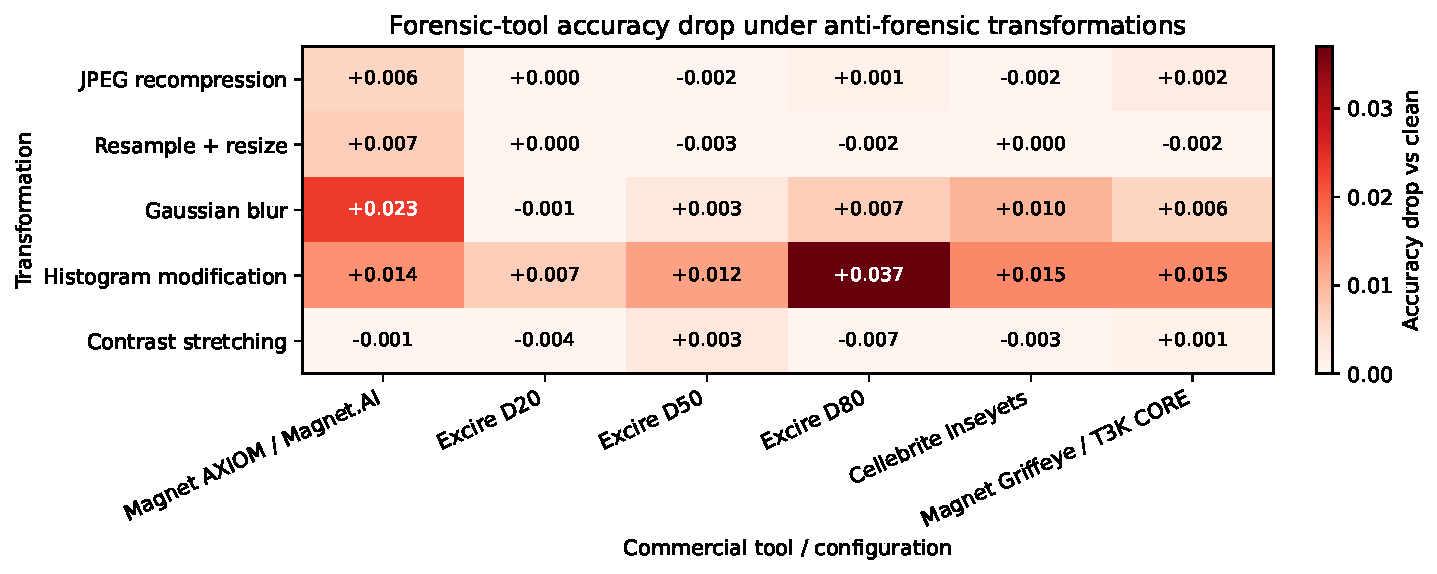
\includegraphics[width=0.95\textwidth]{images/fig_forensic_tools_anti_forensic_accuracy_drop_heatmap.pdf}
\caption{Accuracy drop of commercial black-box tools under anti-forensic transformations.}
\label{fig:results-forensic-tools-antiforensic-drop-heatmap}
\end{figure}

Figure~\ref{fig:results-forensic-tools-antiforensic-drop-heatmap} complements
the tabular interpretation by showing that, for commercial tools,
anti-forensic transformations generally produce limited drops. The most evident
variations are observed for \gls{excirefoto2025} under the \texttt{D80}
configuration with \gls{histogrammodification} and, to a lesser extent, for
\gls{magnetai} under \gls{gaussianblur}. \gls{griffeye}/\gls{t3kcore} maintains
a limited drop, while still presenting residual false negatives in the most
critical condition.

The anti-forensic results show generally limited degradation in both proxy
models and commercial tools. This result is important because it distinguishes
the operational effect of realistic transformations from the more aggressive
effect of adversarial perturbations. For EfficientNet-B0, the most critical
condition is \gls{gaussianblur}, which produces 17 induced errors, all in the
\texttt{weapon}\(\rightarrow\)\texttt{non\_weapon} direction. Although the
aggregate drop is limited, this error direction is forensically relevant,
because it corresponds to missed detection of images containing weapons.

ResNet18 shows the most marked anti-forensic degradation under
\gls{histogrammodification}, with an accuracy of 0.934 and 39 induced errors.
Unlike EfficientNet-B0, the error pattern is bidirectional: both missed
detections of the \texttt{weapon} class and false \texttt{weapon} flags on
\texttt{non\_weapon} images are present. \gls{clip}, instead, remains relatively
stable with respect to the tested transformations. This confirms that, in the
present protocol, the main criticality of \gls{clip} is not anti-forensic
degradation, but the tendency to absorb \gls{ood} inputs into the
\texttt{weapon} class.

Commercial tools also show limited aggregate degradation.
\gls{griffeye}/\gls{t3kcore} presents the highest aggregate anti-forensic
accuracy, equal to 0.974, followed by \gls{cellebriteinseyets},
\gls{excirefoto2025} under the \texttt{D50} configuration, and \gls{magnetai}.
However, the operational interpretation varies across tools.
\gls{griffeye}/\gls{t3kcore} maintains a very limited \gls{fpr}, but shows
residual false negatives under \gls{histogrammodification}.
\gls{cellebriteinseyets} maintains high recall, but with a higher \gls{fpr}
than \gls{griffeye}/\gls{t3kcore}. \gls{magnetai} is more exposed to false
negatives under \gls{gaussianblur}, whereas \gls{excirefoto2025} shows a
criticality more related to the increase in false positives under
\gls{histogrammodification}.

\paragraph{Robustness with respect to adversarial perturbations.}

Table~\ref{tab:results-comparative-adversarial} summarizes the adversarial
robustness profile. Unlike anti-forensic transformations, adversarial
perturbations are designed to stress the decision behavior of \gls{ai}-based
systems. For this reason, they produce more heterogeneous and more
model-dependent effects. The results highlight an important distinction between
the white-box vulnerability of proxy models and the operational black-box
behavior of commercial tools.

\begin{table}[H]
\centering
\caption{Comparison of robustness under adversarial perturbations.}
\label{tab:results-comparative-adversarial}
\small
\renewcommand{\arraystretch}{1.18}
\setlength{\tabcolsep}{3pt}
\begin{tabularx}{\textwidth}{@{}p{2.7cm} p{1.8cm} p{3.1cm} p{2.8cm} X@{}}
\toprule
\textbf{System} &
\textbf{Adv. acc./drop} &
\textbf{Most critical condition} &
\textbf{Main error} &
\textbf{Robustness interpretation} \\
\midrule

EfficientNet-B0 &
0.695 / 0.283 &
\gls{sigmazero}; acc. 0.015; drop 0.963 &
963 induced errors; 489 W$\rightarrow$NW and 474 NW$\rightarrow$W &
Most marked proxy vulnerability in the white-box scenario; high clean accuracy
does not guarantee adversarial robustness. \\

ResNet18 &
0.955 / 0.009 &
\gls{fgsm}; acc. 0.918; drop 0.046 &
47 induced errors; 27 W$\rightarrow$NW and 20 NW$\rightarrow$W &
More stable adversarial profile than EfficientNet-B0, but with residual
degradation under \gls{fgsm}. \\

\gls{clip} &
0.927 / 0.000 &
\gls{fgsm}; acc. 0.914; drop 0.013 &
23 induced errors; 8 W$\rightarrow$NW and 15 NW$\rightarrow$W &
Limited degradation with respect to the tested attacks; adversarial stability
does not eliminate OOD risk. \\

Magnet AXIOM / Magnet.AI &
0.923 / 0.027 &
\gls{fgsm}; acc. 0.867; FNR 0.192 &
96 FN &
Moderate aggregate robustness, but \gls{fgsm} substantially increases false
negatives on the \texttt{weapon} class. \\

Excire Foto 2025 D50 &
0.904 / 0.040 &
\gls{sigmazero}; acc. 0.742; FPR 0.442 &
221 FP &
The perturbation primarily produces semantic over-triggering, rather than
systematic concealment of \texttt{weapon} images. \\

Cellebrite Inseyets &
0.955 / 0.009 &
\gls{fgsm}; acc. 0.918; FNR 0.106 &
53 FN &
Good aggregate commercial stability even in the adversarial scenario, with an
increase in false negatives especially under \gls{fgsm}. \\

Magnet Griffeye / T3K CORE &
0.969 / 0.009 &
\gls{sigmazero}; acc. 0.959; FNR 0.074 &
37 FN &
Highest aggregate commercial accuracy in the adversarial scenario; the low
\gls{fpr} also reflects the conservative mapping, while residual sensitivity to
sparse perturbations remains. \\

\bottomrule
\end{tabularx}

\vspace{0.4em}
\footnotesize
\textit{Note.} For the proxy models, aggregate values are computed across the
five adversarial perturbations considered. For commercial systems, values derive
from the normalized outputs on the forensic evaluation bundle. The drop is
defined in Section~\ref{sec:results-scope}. W$\rightarrow$NW indicates
transitions from \texttt{weapon} to \texttt{non\_weapon}; FN indicates false
negatives; FNR indicates false negative rate; FPR indicates false positive rate.
\end{table}

\begin{figure}[H]
\centering
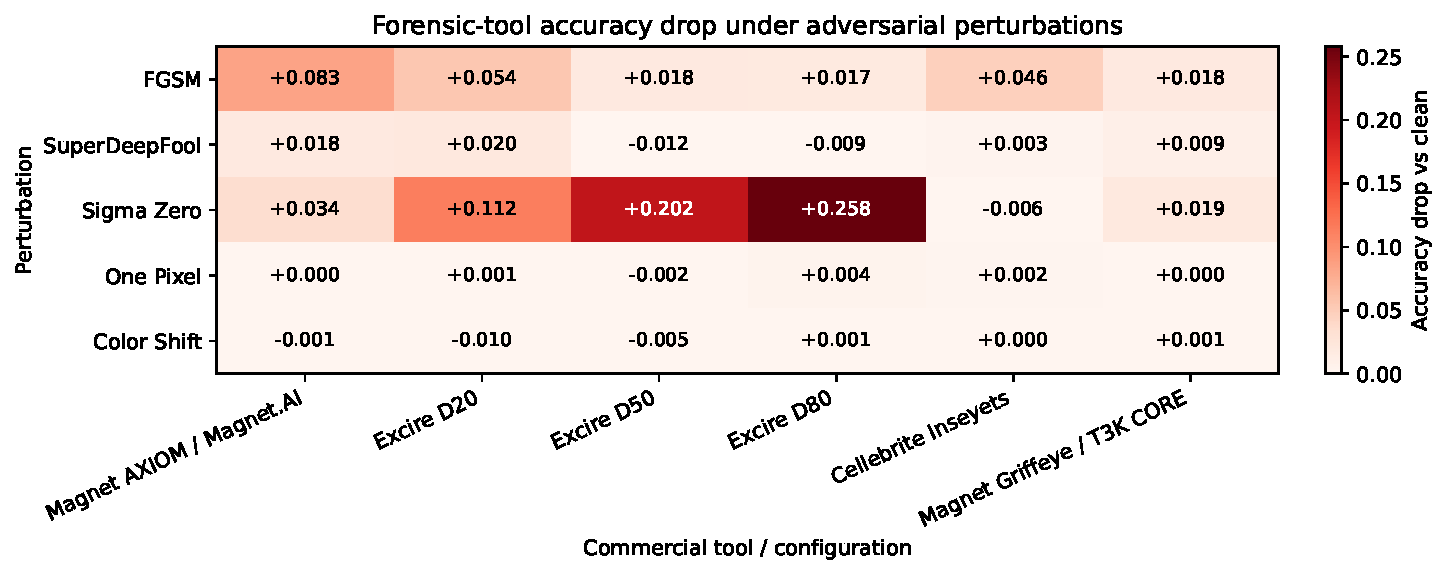
\includegraphics[width=0.95\textwidth]{images/fig_forensic_tools_adversarial_accuracy_drop_heatmap.pdf}
\caption{Accuracy drop of commercial black-box tools under adversarial perturbations.}
\label{fig:results-forensic-tools-adversarial-drop-heatmap}
\end{figure}

Figure~\ref{fig:results-forensic-tools-adversarial-drop-heatmap} shows that the
response of commercial tools to adversarial perturbations is strongly dependent
on the system and configuration. \gls{excirefoto2025} is particularly sensitive
to \gls{sigmazero} under the \texttt{D50} and \texttt{D80} configurations,
whereas \gls{cellebriteinseyets} and \gls{griffeye}/\gls{t3kcore} show more
limited aggregate drops. This result reinforces the interpretation that the
operational robustness of commercial black-box tools is not uniform, but depends
on the type of observable output, the adopted mapping, and the system
configuration.

The adversarial comparison shows that the most severe degradation occurs at the
proxy level, particularly for EfficientNet-B0 under \gls{sigmazero}. The model
moves from a clean accuracy of 0.978 to an accuracy of 0.015, with 963 induced
errors. This result shows, in the considered protocol, that a model may be very
accurate under nominal conditions and, at the same time, extremely fragile with
respect to optimized adversarial perturbations. \gls{fgsm} also produces
significant degradation for EfficientNet-B0, with an accuracy of 0.575 and a
drop of 0.403. The observed vulnerability is therefore not limited to a single
adversarial condition.

ResNet18 and \gls{clip} show a more stable profile in the present experimental
setting. ResNet18 is most affected by \gls{fgsm}, but the drop remains much
lower than that observed for EfficientNet-B0. \gls{clip} is even less degraded
by the tested perturbations. However, this result must be interpreted with
caution: the attacks were not primarily optimized against \gls{clip} as a
white-box target, and \gls{clip} already exhibits a different criticality on
\gls{ood} inputs. Therefore, the adversarial stability observed for \gls{clip}
must not be generalized beyond the evaluated threat model.

Commercial tools show a different pattern. \gls{magnetai} does not reproduce the
catastrophic degradation observed for EfficientNet-B0 under \gls{sigmazero},
but is substantially affected by \gls{fgsm}, with a \gls{fnr} of 0.192. From a
forensic perspective, this is a critical error, because the missed detection of
\texttt{weapon} images may lead to the deprioritization of relevant material.

\gls{excirefoto2025} under the \texttt{D50} configuration instead reacts
differently: \gls{sigmazero} primarily produces an increase in the false
positive rate, equal to 0.442, generating semantic over-triggering rather than
systematic concealment of the \texttt{weapon} class. \gls{cellebriteinseyets}
shows high recall and limited degradation, but maintains a higher false positive
rate than \gls{griffeye}/\gls{t3kcore}. Under the adopted conservative mapping,
\gls{griffeye}/\gls{t3kcore} presents the highest aggregate commercial accuracy
and the lowest false positive rate, while still retaining residual false
negatives on the \texttt{weapon} class.

Overall, the commercial comparison does not identify a single preferable tool
across all operational criteria, but highlights different risk profiles. \gls{griffeye}/\gls{t3kcore}
presents the most selective profile and the lowest operational noise in terms
of false positives; \gls{cellebriteinseyets} maintains slightly higher recall on
the \texttt{weapon} class; \gls{excirefoto2025} shows behavior strongly
dependent on the retrieval threshold; and \gls{magnetai} presents a more
conservative profile but with greater false negative risk. This heterogeneity
confirms that the operational robustness of commercial black-box software is
tool-dependent and must be interpreted with respect to the type of observable
output, the adopted mapping, and the role of the analyst in the workflow.

\paragraph{Threshold sensitivity and black-box interpretation.}

The results of \gls{excirefoto2025} require a separate interpretation, because
the system was evaluated as a semantic retrieval engine and not as a native
forensic classifier. The \texttt{Distance limit} parameter defines the
operational restrictiveness of semantic retrieval. The \texttt{D20}
configuration is restrictive: it reduces false positives and weapon flags on
\gls{ood} inputs, but increases the risk of missed detection of \texttt{weapon}
images. The \texttt{D80} configuration is permissive: it maximizes recall, but
increases false positives and the assignment of non-relevant or perturbed images
to the semantic query related to weapons. The \texttt{D50} configuration was
used as the main comparison point because it represents an intermediate profile.

This threshold dependence is particularly evident under \gls{sigmazero}. Under
the \texttt{D20} configuration, \gls{excirefoto2025} achieves an accuracy of
0.815, an FNR of 0.180, and an FPR of 0.190. Under the \texttt{D50}
configuration, accuracy decreases to 0.742, while FNR improves to 0.074 and FPR
increases to 0.442. Under the \texttt{D80} configuration, recall improves
further, but FPR rises to 0.662. The same tool can therefore support different
forensic priorities depending on the selected operating point: \texttt{D20} is
more suitable for containing noise, \texttt{D80} for maximizing recall, and
\texttt{D50} for balancing false negatives and false positives.

The black-box nature of commercial tools also limits the type of conclusions
that can be formulated. Unlike the proxy models, these systems do not expose
decision boundaries, calibrated scores, architectures, training data, or
internal thresholding logic. Their outputs can therefore be evaluated only at
the operational level, through observable categories, exported tags, retrieval
results, semantic bookmarks, matching rate, non-mappable outputs, false
negatives, false positives, and behavior on \gls{ood} inputs. This limitation
does not represent a weakness of the evaluation protocol; on the contrary, it
reflects the real condition in which forensic analysts interact with
\gls{ai}-assisted commercial tools.

\paragraph{Overall operational interpretation.}

The comparative analysis confirms that robustness in \gls{ai}-assisted forensic
image triage is a multidimensional property. Clean accuracy measures nominal
performance, but it does not capture \gls{ood} input absorption, sensitivity to
perturbations, false negative risk, semantic over-triggering, or the effect of
thresholds in black-box systems. In \gls{df} workflows, these dimensions are at
least as relevant as aggregate accuracy, because they influence analyst
attention, content prioritization, and the manual review strategy.

Three main findings emerge. First, proxy models are useful because they make
controlled degradation patterns observable and allow confidence shift, induced
errors, and error direction to be measured. However, their behavior cannot be
automatically transferred to commercial tools, which adopt proprietary
mechanisms for classification, tagging, retrieval, or semantic bookmark
generation. Second, commercial tools show differentiated risk profiles: some
privilege recall, others reduce false positives, and others depend strongly on
the retrieval configuration or the adopted semantic mapping. Third, \gls{ood}
behavior remains an autonomous risk: it may increase the analyst's workload,
produce misleading prioritization, and generate weapon-related flags on material
that does not belong to the expected binary task.

Overall, the results support a cautious interpretation of \gls{ai}-based
automation in forensic contexts. The evaluated systems can provide useful
support for triage, prioritization, and large-scale review of multimedia
content. However, their outputs must not be treated as conclusive evidence or as
substitutes for expert validation. In particular, missed detections of
\texttt{weapon} images, high-confidence OOD assignments, and threshold-dependent
errors must be explicitly documented when \gls{ai}-assisted tools are used in
forensic workflows. The \textsc{FAIR-Lab} protocol responds to this need by
combining frozen datasets, traceable manifests, hash-based reproducibility,
controlled perturbation families, black-box output normalization, and manual
auditability of the final interpretation.


% ─────────────────────────────────────────────────────────────────────────────
\section{Explainability Analysis and Representative Failure Cases}
\label{sec:results-xai}
% ─────────────────────────────────────────────────────────────────────────────

The \gls{xai} analysis was used as a qualitative and diagnostic tool to connect
the aggregate metrics discussed in the previous sections to a restricted set of
representative cases. It does not constitute a primary robustness metric and
does not replace quantitative measures of accuracy, confidence, false positives,
and false negatives. Its role is instead to support the operational
interpretation of selected behaviors observed in the proxy model, by highlighting
which image regions contributed to the classifier decision in specific success
or failure scenarios.

The attribution maps were generated using \gls{ig} on the white-box
EfficientNet-B0 proxy model, using the model-predicted class as the attribution
target, indicated in the experimental files as \texttt{predicted\_label}. This
choice makes it possible to analyze not what the model should have recognized
according to the manual label, but what actually guided the decision it
produced. Consequently, in erroneous cases, the visualization is oriented toward
understanding which visual elements supported the incorrect classification.

The generated maps must not be interpreted as direct explanations of the
behavior of \gls{magnetaxiomtool}/\gls{magnetai},
\gls{excirefoto2025}, \gls{cellebriteinseyets}, or
\gls{griffeye}/\gls{t3kcore}, which remain black-box systems in the context of
this evaluation. Rather, they provide a controlled diagnostic reference, limited
to the white-box proxy model, that is useful for discussing in more concrete
terms selected operational risks observable in a \gls{df}
\textit{human-in-the-loop} context.

The XAI figures reported in this section follow the structure introduced in
Chapter~\ref{chap:methodology}: input image, \gls{ig} heatmap, attribution
overlay on the original image, and mask of the regions with the highest
attribution. Unlike the methodological example, the visualizations are used here
to discuss representative cases from the experimental evaluation. The
attribution mask must not be interpreted as a semantic segmentation or as object
ground truth, but as a visual summary of the areas that most contributed to the
proxy model prediction. Similarly, the reported confidence is the proxy model
score and not a calibrated probability.

Table~\ref{tab:results-xai-cases} summarizes the five cases selected for the
qualitative analysis. The selection covers one correct case on a clean input,
one false negative on a clean input, one \gls{ood} case classified as
\texttt{weapon}, one false negative produced by an anti-forensic transformation,
and one high-confidence adversarial false positive.

\begin{table}[htbp]
\centering
\small
\renewcommand{\arraystretch}{1.15}
\begin{tabular}{p{0.18\textwidth} p{0.18\textwidth} p{0.15\textwidth} p{0.15\textwidth} p{0.22\textwidth}}
\toprule
\textbf{Identifier} &
\textbf{Scenario} &
\textbf{Manual label} &
\textbf{Prediction} &
\textbf{Operational role} \\
\midrule

\texttt{xai\_case\_0001} &
\texttt{clean} &
\texttt{weapon} &
\texttt{weapon} &
Correct case on a clean input, used as a reference for observing coherent
attribution behavior. \\

\texttt{xai\_case\_0006} &
\texttt{clean} &
\texttt{weapon} &
\texttt{non\_weapon} &
False negative on a clean input, representative of missed detection in the
absence of perturbations. \\

\texttt{xai\_case\_0009} &
\texttt{ood} &
\texttt{ood} &
\texttt{weapon} &
\gls{ood} sample classified as \texttt{weapon}, representative of the risk of
improper semantic inclusion. \\

\texttt{xai\_case\_0010} &
\gls{histogrammodification} &
\texttt{weapon} &
\texttt{non\_weapon} &
Anti-forensic false negative, representative of the effects of low-level visual
manipulations. \\

\texttt{xai\_case\_0015} &
\gls{sigmazero} &
\texttt{non\_weapon} &
\texttt{weapon} &
High-confidence adversarial false positive, representative of the unreliability
of confidence alone in the presence of an attack. \\

\bottomrule
\end{tabular}
\caption{Representative cases selected for the qualitative analysis of EfficientNet-B0 using \gls{ig}.}
\label{tab:results-xai-cases}
\end{table}

\XAIcaseFigureMaskGrid
{fig:xai-case1-clean-correct}
{Correct case on a clean input \texttt{xai\_case\_0001}. The EfficientNet-B0
proxy model correctly classifies a \texttt{clean} image with manual label
\texttt{weapon} as \texttt{weapon}.}
{images/fig_xai_case1_clean_correct_input.png}
{images/fig_xai_case1_clean_correct_heatmap.png}
{images/fig_xai_case1_clean_correct_overlay.png}
{images/fig_xai_case1_clean_correct_top10_mask.png}
{\textbf{scenario}: \texttt{clean};
 \textbf{manual label}: \texttt{weapon};
 \textbf{prediction}: \texttt{weapon};
 \textbf{confidence}: 1.000}

The first case, shown in Figure~\ref{fig:xai-case1-clean-correct}, provides a
qualitative reference in which the model prediction is consistent with the
manual label. The image belongs to the \texttt{clean} scenario, the expected
class is \texttt{weapon}, and the prediction produced by EfficientNet-B0 is also
\texttt{weapon}, with very high confidence. In this case, the \gls{ig} map is
useful for verifying whether the attribution pattern is compatible with the
visually relevant region of the image, rather than being dominated by marginal
elements, background, or acquisition artifacts. This example does not, by
itself, demonstrate the general reliability of the model, but constitutes a
reference case against which the subsequent failures can be compared.

\XAIcaseFigureMaskGrid
{fig:xai-case2-clean-false-negative}
{False negative on a clean input \texttt{xai\_case\_0006}. A \texttt{clean}
image with manual label \texttt{weapon} is classified as
\texttt{non\_weapon}.}
{images/fig_xai_case2_clean_false_negative_input.png}
{images/fig_xai_case2_clean_false_negative_heatmap.png}
{images/fig_xai_case2_clean_false_negative_overlay.png}
{images/fig_xai_case2_clean_false_negative_top10_mask.png}
{\textbf{scenario}: \texttt{clean};
 \textbf{manual label}: \texttt{weapon};
 \textbf{prediction}: \texttt{non\_weapon};
 \textbf{confidence}: 0.692}

The second case, reported in
Figure~\ref{fig:xai-case2-clean-false-negative}, is relevant because the error
occurs on a clean input, without adversarial perturbations or anti-forensic
transformations. The image is manually labeled as \texttt{weapon}, but
EfficientNet-B0 classifies it as \texttt{non\_weapon} with moderate confidence.
In a \gls{df} workflow, this type of error may produce a concrete operational
risk, since a false negative may prevent a potentially relevant image from being
prioritized during automated triage.

The corresponding \gls{ig} map makes it possible to observe whether the model
decision is supported by genuinely relevant regions or whether the attribution
appears dispersed, partial, or influenced by contextual elements. This case
shows that good aggregate performance on \texttt{clean} data does not eliminate
the need for human assessment, especially when the automatic result is used to
filter or rank large volumes of images in an investigative context.

\XAIcaseFigureMaskGrid
{fig:xai-case3-ood-as-weapon}
{\gls{ood} case \texttt{xai\_case\_0009}. An out-of-distribution sample is
classified as \texttt{weapon} with high confidence.}
{images/fig_xai_case3_ood_as_weapon_input.png}
{images/fig_xai_case3_ood_as_weapon_heatmap.png}
{images/fig_xai_case3_ood_as_weapon_overlay.png}
{images/fig_xai_case3_ood_as_weapon_top10_mask.png}
{\textbf{scenario}: \texttt{ood};
 \textbf{manual label}: \texttt{ood};
 \textbf{prediction}: \texttt{weapon};
 \textbf{confidence}: 0.999}

The third case, shown in Figure~\ref{fig:xai-case3-ood-as-weapon}, illustrates a
risk that differs from an ordinary false positive. The sample is labeled as
\texttt{ood}, but it is absorbed by the binary decision boundary and classified
as \texttt{weapon} with high confidence. This behavior is particularly important
because \gls{ood} inputs do not simply correspond to realistic negatives, but
include borderline, anomalous, degraded, synthetic, or semantically
out-of-distribution cases with respect to the main task.

The \gls{ig} visualization makes it possible to inspect whether the decision is
associated with localized regions that the model interprets as compatible with
features of the \texttt{weapon} class, or whether it emerges from more diffuse
and less semantically stable correlations. From a methodological perspective,
this case supports the choice to treat \texttt{ood} as an autonomous category in
dataset construction and in the evaluation of operational robustness, rather
than mapping all inputs not belonging to the \texttt{weapon} class to the
\texttt{non\_weapon} class alone.

\XAIcaseFigureMaskGrid
{fig:xai-case4-antiforensic-failure}
{Anti-forensic false negative \texttt{xai\_case\_0010}. A \texttt{weapon} image
subjected to \gls{histogrammodification} is classified as
\texttt{non\_weapon}.}
{images/fig_xai_case4_antiforensic_failure_input.png}
{images/fig_xai_case4_antiforensic_failure_heatmap.png}
{images/fig_xai_case4_antiforensic_failure_overlay.png}
{images/fig_xai_case4_antiforensic_failure_top10_mask.png}
{\textbf{scenario}: \gls{histogrammodification};
 \textbf{manual label}: \texttt{weapon};
 \textbf{prediction}: \texttt{non\_weapon};
 \textbf{confidence}: 0.870}

The fourth case, reported in
Figure~\ref{fig:xai-case4-antiforensic-failure}, concerns an anti-forensic
transformation based on \gls{histogrammodification}. The manual label remains
\texttt{weapon}, but the model predicts \texttt{non\_weapon} with high
confidence. The case is relevant because the transformation does not represent
only an abstract adversarial perturbation optimized against a differentiable
model, but a low-level visual manipulation that may affect tonal distribution,
contrast, and the local perception of image structures.

The \gls{ig} map makes it possible to observe whether the histogram modification
alters the regions that contribute to the model decision, reducing the weight
assigned to the object of interest or shifting attention toward less informative
areas. From an operational perspective, this failure suggests that
transformations that may still be compatible with human recognizability of the
content can nevertheless compromise automated classification. In a forensic
pipeline, this reinforces the need not to treat the classifier output as
autonomous evidence, but as support to be critically verified.

\XAIcaseFigureMaskGrid
{fig:xai-case5-adversarial-high-confidence-failure}
{High-confidence adversarial false positive \texttt{xai\_case\_0015}. A
\texttt{non\_weapon} image perturbed using \gls{sigmazero} is classified as
\texttt{weapon}.}
{images/fig_xai_case5_adversarial_high_conf_failure_input.png}
{images/fig_xai_case5_adversarial_high_conf_failure_heatmap.png}
{images/fig_xai_case5_adversarial_high_conf_failure_overlay.png}
{images/fig_xai_case5_adversarial_high_conf_failure_top10_mask.png}
{\textbf{scenario}: \gls{sigmazero};
 \textbf{manual label}: \texttt{non\_weapon};
 \textbf{prediction}: \texttt{weapon};
 \textbf{confidence}: 1.000}

The fifth case, shown in
Figure~\ref{fig:xai-case5-adversarial-high-confidence-failure}, represents a
high-confidence adversarial false positive. The image has manual label
\texttt{non\_weapon}, but, after the \gls{sigmazero} perturbation, it is
classified as \texttt{weapon} with a confidence of 1.000. For the purposes of
this thesis, this case is particularly significant because it separates two
concepts that may be incorrectly conflated in an operational workflow: model
confidence and forensic reliability of the prediction.

The \gls{ig} visualization provides a diagnostic representation of the regions
supporting the incorrect decision, but it must not be interpreted as a complete
explanation of the attack mechanism. Its value lies in making a high-confidence
failure inspectable, showing that an apparently certain prediction may still
derive from unreliable input conditions. In an investigative context, this
result supports the need to maintain the \textit{human-in-the-loop} paradigm,
especially when \gls{ai}-based systems are used to prioritize sensitive or
potentially relevant content.

Overall, the five selected cases show that \gls{xai} analysis can provide a
useful interpretive contribution, provided that its role remains correctly
delimited. The correct case on a clean input provides a qualitative reference of
coherent attribution; the false negative on a clean input shows that missed
detection can occur even in the absence of manipulation; the \gls{ood} case
highlights the risk of absorbing out-of-distribution inputs into the
\texttt{weapon} class; the anti-forensic case shows that low-level visual
transformations can alter the automatic decision; and the high-confidence
adversarial case shows that confidence cannot be assumed as a sufficient
indicator of operational reliability.

For these reasons, \gls{xai} analysis is considered in this thesis as support
for understanding representative cases and not as autonomous evidence of system
robustness. It makes selected behaviors of the EfficientNet-B0 proxy model more
transparent, but it does not automatically extend its conclusions to commercial
black-box tools. In a \gls{df} pipeline, visualizations based on \gls{ig} must
therefore be interpreted as tools supporting review, evaluation, and critical
discussion of the results, while preserving the central role of the human
analyst in the final assessment.


% ─────────────────────────────────────────────────────────────────────────────
\section{Operational Interpretation and Experimental Limitations}
\label{sec:results-implications}
% ─────────────────────────────────────────────────────────────────────────────

The results of Chapter~\ref{chap:results} show that the operational robustness
of \gls{ai}-based systems for forensic image triage cannot be inferred from
clean accuracy alone. The interpretation must jointly consider the direction of
errors, behavior on \gls{ood} inputs, sensitivity to perturbations, the
operational configuration of the tools, normalization of black-box outputs, and
the availability of human review.

From a forensic perspective, the most relevant point is that performance
degradation does not always have the same operational meaning. A false negative
on the \texttt{weapon} class may prevent investigatively relevant content from
being submitted to review; a false positive or a weapon flag on \gls{ood}
content may instead increase the triage workload and generate improper
priorities. For this reason, the most significant evidence in this chapter
concerns the observed failure modes, rather than only the aggregate value of
accuracy.

The evaluation of commercial tools must be interpreted with particular caution:
\gls{magnetaxiomtool}/\gls{magnetai}, \gls{excirefoto2025},
\gls{cellebriteinseyets}, and \gls{griffeye}/\gls{t3kcore} are evaluated through
observable outputs and documented mapping rules, not through access to internal
models, thresholds, or proprietary decision logic. The commercial comparison is
therefore an operational comparison on the forensic evaluation bundle, not a
general validation of the products and not a comparison among homogeneous
classifiers.

The main methodological limitations---model-dependent attacks generated with
respect to EfficientNet-B0, the non-exhaustive space of anti-forensic
transformations, bundle-weighted commercial metrics, and residual sensitivity to
embedded metadata---are addressed systematically in
Chapter~\ref{chap:conclusions}, together with the methodological, operational,
and legal implications of using \gls{ai}-assisted tools in \gls{df} workflows.
